\documentclass{article}
\usepackage[utf8]{inputenc}
\usepackage[a4paper, margin=2.5cm]{geometry}
\usepackage{graphicx} 
\usepackage{natbib}
\usepackage[french]{babel}

%\usepackage[default,scale=0.95]{opensans}
\usepackage[T1]{fontenc}
\usepackage{amssymb} %math
\usepackage{amsmath}
\usepackage{amsthm}
\usepackage{systeme}
\usepackage{bbm}
\usepackage{media9}
\usepackage{makecell}
\usepackage{url}
\usepackage{minted}
\usepackage{xcolor}
\usepackage{wrapfig}
\usepackage{csquotes}
\usepackage{subcaption}
\usepackage{float}
\usepackage{dirtree}

% \usepackage{lineno}
% \linenumbers

\usepackage{hyperref}
\hypersetup{
    % colorlinks=true,
    % linkcolor=blue,
    % filecolor=magenta,      
    % urlcolor=cyan,
    pdftitle={Projet ML},
    %pdfpagemode=FullScreen,
    }
\urlstyle{same} %\href{url}{Text}

\renewcommand{\baselinestretch}{1.5}
\graphicspath{{./src/}}

\begin{document}

\begin{titlepage}
    \begin{center}
        \vspace*{1cm}

        \Huge
        \textbf{ML - Projet}

        %\vspace{0.5cm}
        \LARGE
        Réseau de neurones : DIY

        %\vspace{1.5cm}
        \Large
        Charles \textsc{Vin}, Aymeric \textsc{Delefosse}

        \vfill
        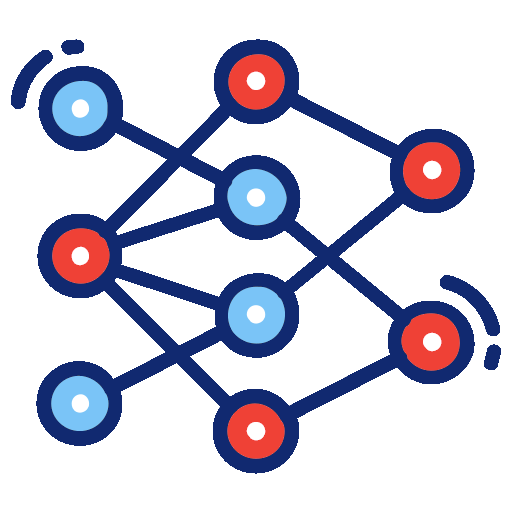
\includegraphics[width=.5\textwidth]{neural-network.png}    
        \vfill

        \large
        DAC | 2022-2023 \hfill 
        
\includegraphics[width=0.30\textwidth]{logo.png}
        \hfill
        
        
    \end{center}
\end{titlepage}

\tableofcontents
\newpage

\section{Introduction}

Ce projet, réalisé entièrement en Python et aux concepts algébriques, avait pour objectif de développer une bibliothèque de \textit{deep learning}. À travers des expérimentations significatives, nous avons exploré diverses tâches telles que la reconstruction d'images, la génération de données et l'entraînement de réseaux convolutionnels. Ces expérimentations nous ont permis d'analyser l'impact des choix architecturaux, des techniques d'optimisation, des hyperparamètres et des contraintes matérielles sur les performances des modèles. Ce projet a ainsi contribué à approfondir notre compréhension du \textit{machine learning}.

\textbf{Note} : n'hésitez pas à zoomer sur les figures !

\section{Implémentation}

Le code est disponible sur \href{https://github.com/dataymeric/NeuralNetworksDIY}{ce dépôt GitHub}.

\begin{itemize}
    \item Implémentation optimisée de la convolution avec le moins de boucles possibles (utilisation de fonctions avancées de \texttt{numpy}); 
    \item Une documentation en ligne ;
    \item Implémentation d'un \texttt{logger} qui peut afficher graphiquement la \textit{loss} après chaque époque ; 
    \item Early stopping qui permet de réduire les temps d'apprentissage et les risques de sur-apprentissage.
\end{itemize}

La bibliothèque est organisée de manière analogue aux bibliothèques de \textit{deep learning} plus populaires.

\section{Expérimentation}

Dans le but de mettre notre bibliothèque à l'épreuve, nous avons entrepris une série d'expérimentations en utilisant diverses architectures sur deux types de données distincts. Le premier ensemble de données était constitué de jeux aléatoires de données gaussiennes, présentant des caractéristiques linéairement séparables ou non, tels que le XOR ou le jeu d'échecs. Le second ensemble de données concernait la classification d'images sur deux jeux de données : un pour la reconnaissance de chiffres (le plus populaire : \texttt{USPS}) et le deuxième, plus complexe, pour la reconnaissance de vêtements (\texttt{Fashion MNIST}).

\subsection{Classification}

\subsubsection{Effet de l'initialisation des paramètres}

Nous avons très vite constaté le rôle et l'impact de l'initialisation des paramètres sur les performances des réseaux de neurones. Cette initialisation peut paraître anodine à première vue mais joue un rôle crucial sur la performance et la significativité du modèle. \\
Une initialisation inadéquate peut entraîner des problèmes tels que la saturation des neurones, la divergence de l'apprentissage ou la stagnation dans des minima locaux. Une initialisation judicieuse peut quant à elle favoriser une convergence plus rapide et une meilleure généralisation des données. \\
Ainsi, l'optimisation des poids et des biais à l'initialisation constitue une étape cruciale dans la conception et l'entraînement des réseaux de neurones. Cette initialisation peut se faire en prenant en compte les spécificités de l'architecture et de la fonction d'activation.

Ainsi, pour les modules utilisant des paramètres (linéaire et convolution), il est possible d'initialiser les poids et biais de huit manières différentes :

\begin{itemize}
    \item Initialisation normale : les paramètres sont initialisés selon une loi normale centrée réduite : $ W, B \sim \mathcal{N}(0, 1) $ ;
    \item Initialisation uniforme : les paramètres sont initialisés selon une loi uniforme : $ W, B \sim \mathcal{U}(0, 1) $ ;
    \item Initialisation à 1 : tous les paramètres sont initialisés à 1 ;
    \item Initialisation à 0 : tous les paramètres sont initialisés à 0 ;
    \item Initialisation de Xavier (ou de Glorot) : cette méthode, développée par Xavier Glorot et Yoshua Bengio, ajuste les poids de manière à maintenir une variance constante tout au long du réseau, en fonction du nombre d'entrées et de sorties de chaque couche. Cela favorise une propagation efficace du signal. Il est possible d'initialiser selon une loi normale ou une loi uniforme, où $ \text{input} $ représente la taille de l'entrée dans le cadre d'un module linéaire, le nombre de canaux d'entrée dans le cadre d'une convolution et $ \text{output} $ représente la taille de la sortie dans le cadre d'un module linéaire, le nombre de canaux en sortie (le nombre de \textit{feature maps}) dans le cadre d'une convolution.
    \begin{itemize}
        \item Loi normale : $ W, B \sim \mathcal{N}(0, \, \sqrt[]{\frac{2}{\text{input} + \text{output}}}) $ ;
        \item Loi uniforme : $ W, B \sim \mathcal{U}(- \sqrt[]{\frac{6}{\text{input} + \text{output}}}, \, \sqrt[]{\frac{6}{\text{input} + \text{output}}}) $.
    \end{itemize}
    \item Initialisation de He (ou de Kaiming) : Cette méthode, développée par Kaiming He et al., est similaire à l'initialisation de Xavier, mais elle prend en compte la variance spécifique des fonctions d'activation asymétriques, telles que la fonction ReLU. Elle permet une initialisation adaptée aux architectures utilisant ces fonctions d'activation. 
    \begin{itemize}
        \item Loi normale : $ W, B \sim \mathcal{N}(0, \, \sqrt[]{\frac{2}{\text{input}}}) $ ;
        \item Loi uniforme : $ W, B \sim \mathcal{U}(- \sqrt[]{\frac{6}{\text{input}}}, \, \sqrt[]{\frac{6}{\text{input}}}) $.
    \end{itemize}
\end{itemize}

\textbf{Note} : pour le module linéaire, les biais sont initialisés par défaut tandis que pour la convolution, les biais sont désactivés par défaut (sauf indication contraire).

Pour évaluer l'effet de l'initialisation des paramètres, nous avons mis en place un réseau simple pour classer le jeu de données \texttt{fashion-mnist}. Ce réseau se compose d'une couche linéaire qui prend en entrée l'image complète et effectue la classification avec dix neurones en sortie. Nous représentons ce réseau sous la forme suivante : \texttt{Linear(784, 10) $ \rightarrow $ Sigmoid()}.

\begin{figure}[htbp]
    \centering
    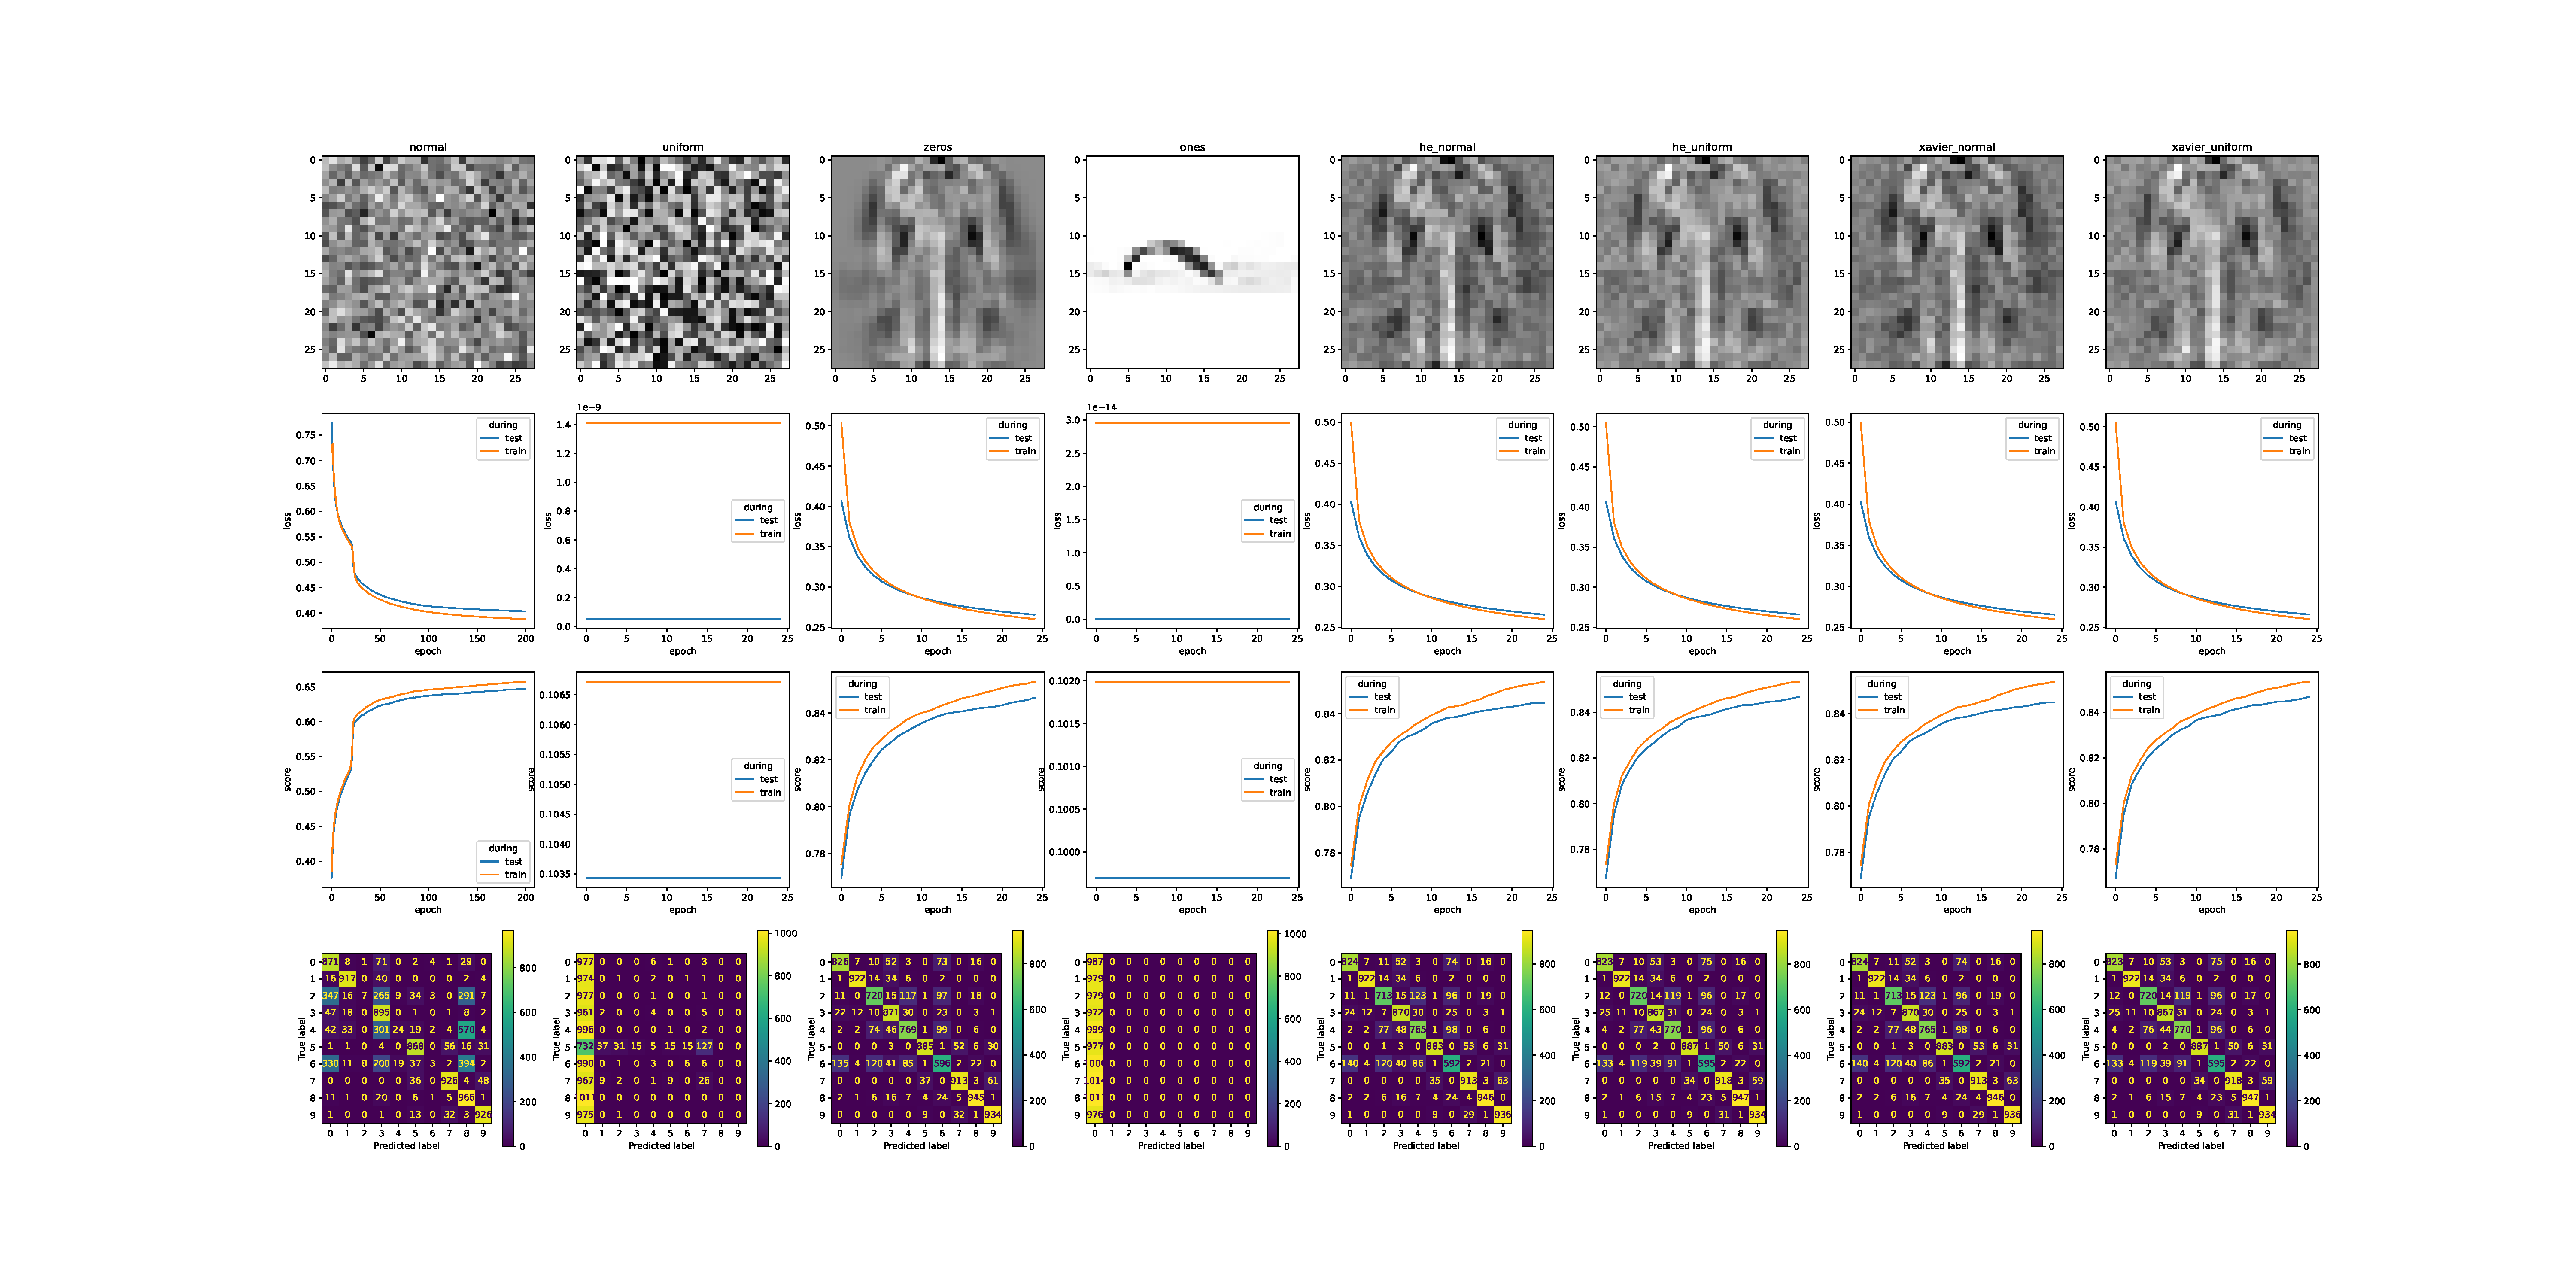
\includegraphics[width=\textwidth]{init_type.pdf}
    \caption{Représentation des paramètres, d'une matrice de confusion, de l'évolution du coût et du score par époque en fonction de l'initialisation des paramètres}
    \label{fig:initparam}
\end{figure}

La figure \ref{fig:initparam} présente les résultats de cette expérimentation. Nous observons des difficultés d'apprentissage avec certaines initialisations. L'initialisation normale conduit à un minimum local (après 200 époques). Les initialisations uniforme et à 1 provoquent une explosion du gradient, empêchant tout apprentissage.

Cette expérience met en évidence l'importance de l'initialisation des paramètres. Il serait peut-être possible de résoudre les problèmes liés à l'initialisation normale en utilisant un autre algorithme d'optimisation, tel que Adam.

\subsubsection{Effet du taux d'apprentissage (\textit{learning rate})}

Le \textit{learning rate} est un hyperparamètre crucial dans l'entraînement des réseaux de neurones. Il contrôle la taille des pas que l'algorithme d'optimisation effectue lors de la mise à jour des poids du réseau pendant l'apprentissage. Un taux d'apprentissage adapté permet aux mises à jour de poids d'être suffisamment grandes pour converger rapidement vers un minimum, tout en évitant les oscillations et les divergences. Le but est donc de trouver un bon compromis entre la rapidité de convergence et la stabilité des résultats.

\begin{figure}[htbp]
    \centering
    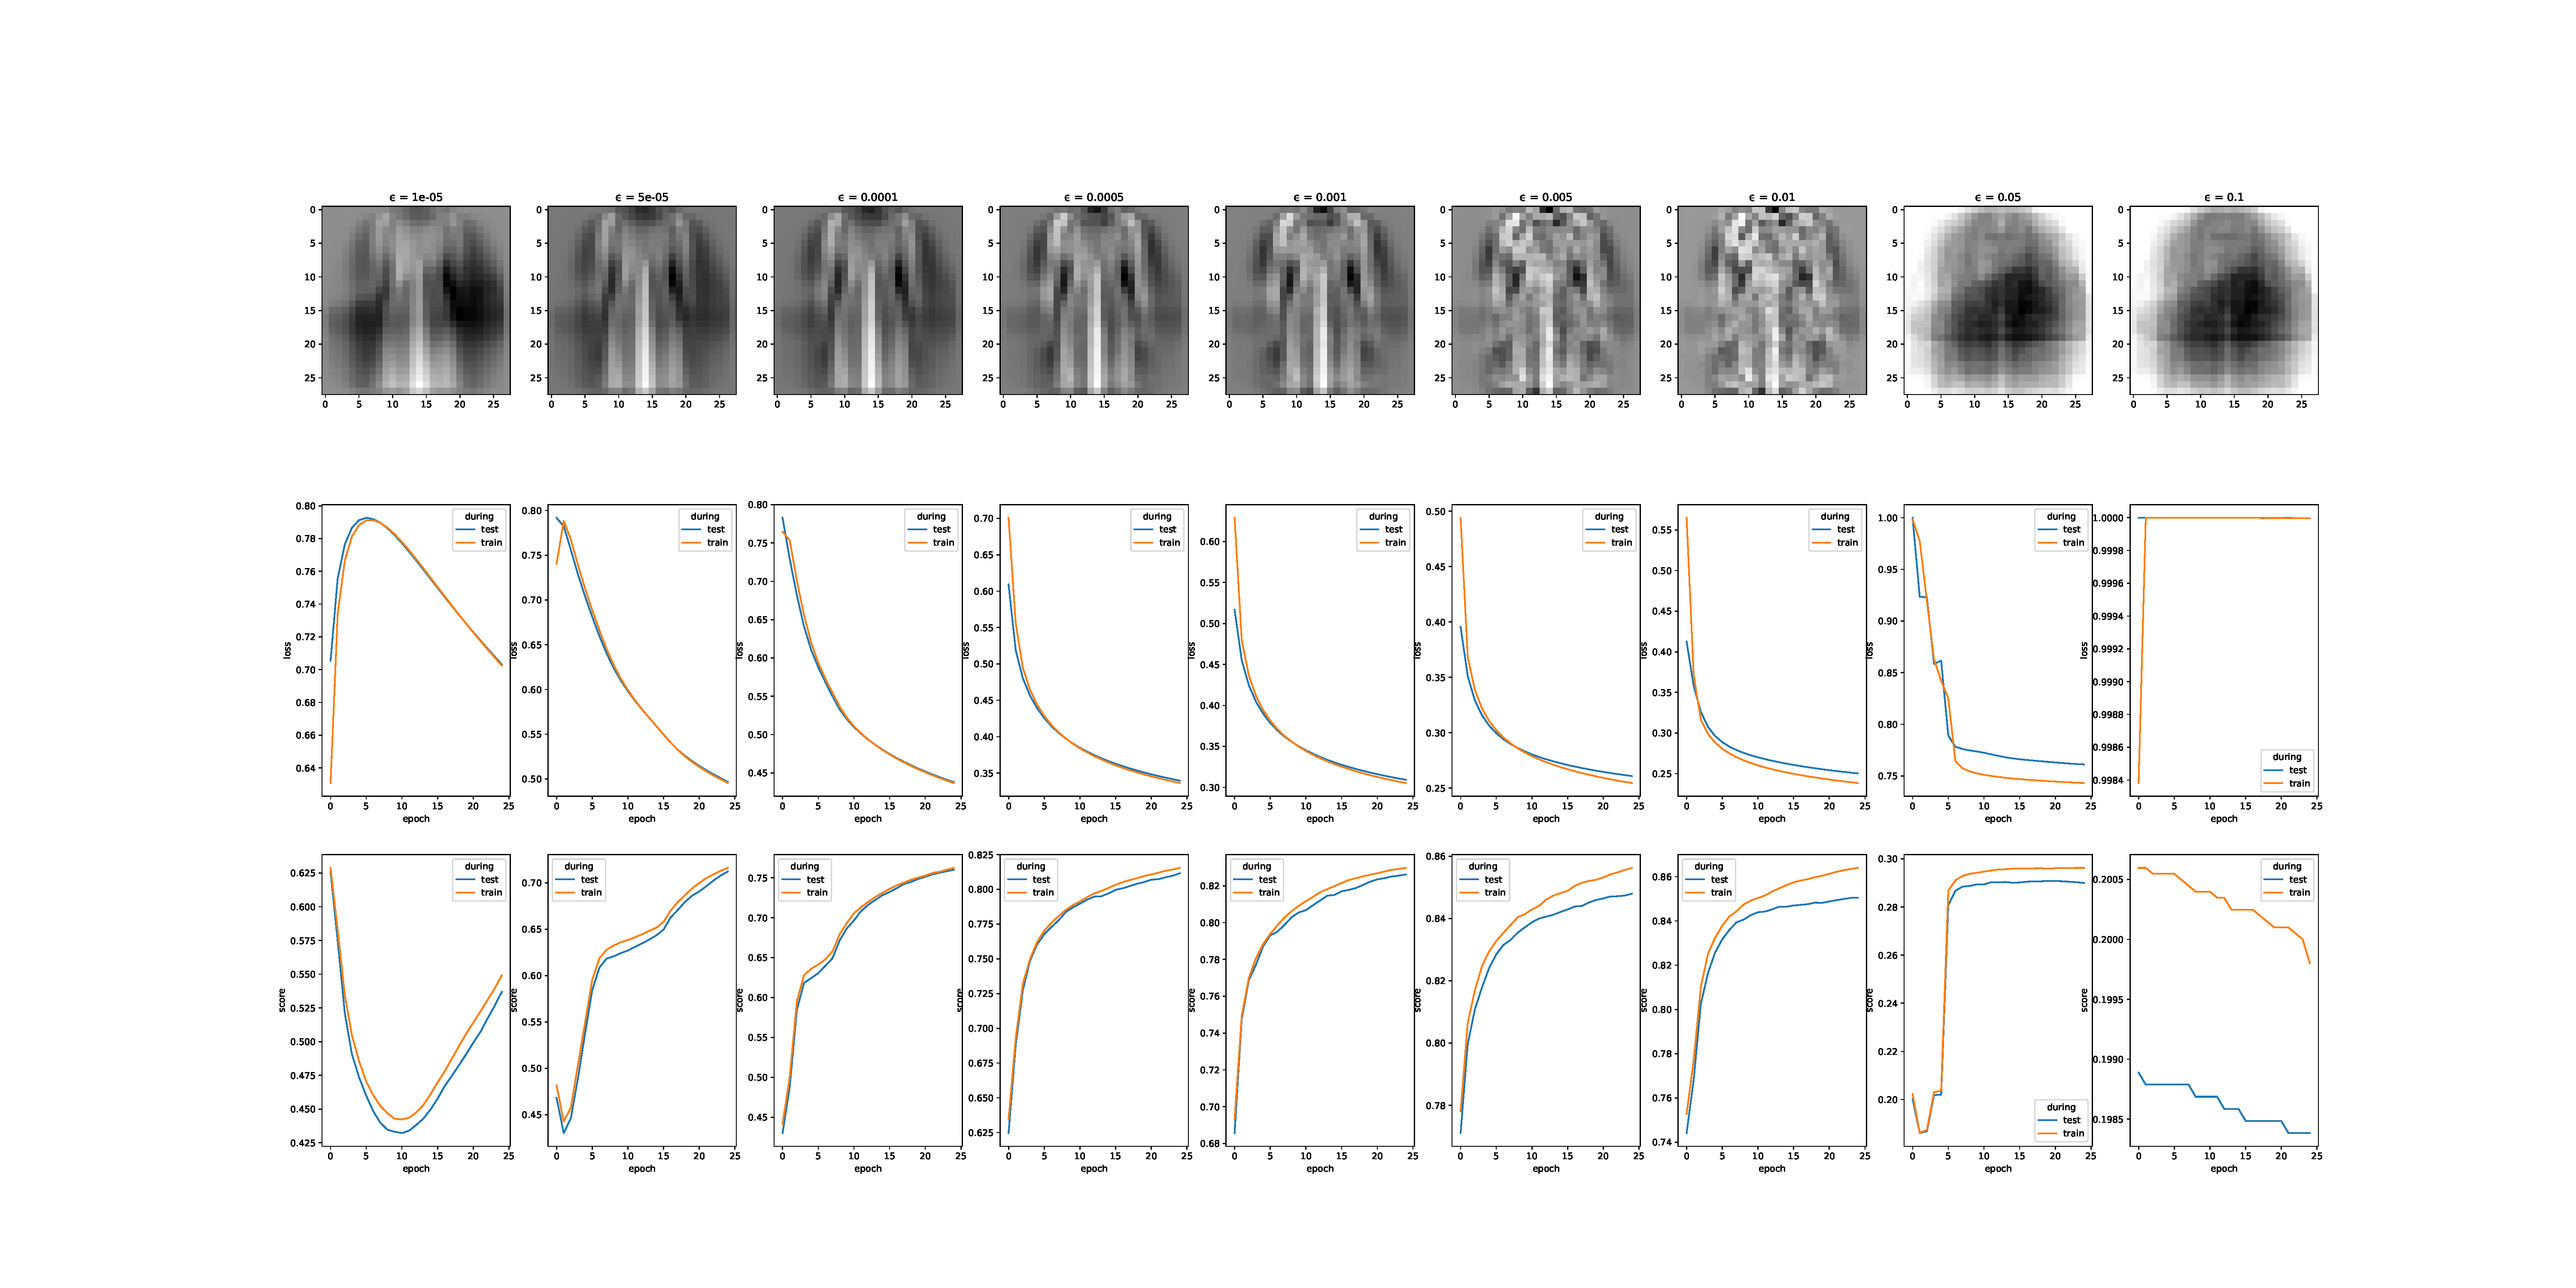
\includegraphics[width=\textwidth]{lr_effet.pdf}
    \caption{Représentation des paramètres, de l'évolution du coût et du score par époque en fonction du taux d'apprentissage $ \epsilon $}
    \label{fig:effetlearningrate}
\end{figure}

Toujours avec le même réseau très simple, nous obtenons les résultats dans la figure \ref{fig:effetlearningrate}. Un \textit{learning rate} trop faible ralentit donc la convergence, et un nombre élevé d'itérations sera nécessaire pour atteindre une performance obtenue avec un taux d'apprentissage plus élevé. Les ajustements apportés aux poids sont également plus lents et progressifs, au risque de rester coincer dans des minima locaux peu optimaux. Un \textit{learning rate} trop élevé entraîne une divergence dans notre cas, les poids se mettent à jour trop brutalement entraînant une convergence vers un modèle très rapidement sous-optimal.

\subsubsection{Effet des fonctions d'activation}

L'ajout d'une fonction d'activation non linéaire après un module linéaire, tel qu'une couche dense ou une convolution, permet d'introduire des interactions non linéaires entre les neurones et d'augmenter la capacité de représentation du modèle. Sans fonction d'activation, le réseau de neurones se réduirait simplement à une combinaison linéaire des entrées, limitant ainsi sa capacité à modéliser des relations complexes.

Différentes fonctions d'activation peuvent être utilisées en fonction du problème et des caractéristiques des données. Par exemple :

\begin{itemize}
    \item La fonction tangente hyperbolique qui comprime les sorties entre -1 et 1 ;
    \item La fonction sigmoïde qui comprime les sorties entre 0 et 1 ;
    \item La fonction sigmoïde "stable" qui a été implémentée dans l'optique d'éviter des instabilités numériques ;
    \item La fonction softmax pour transformer les données en une distribution de probabilités ;
    \item La fonction log-softmax afin d'éviter des instabilités numériques ;
    \item La fonction ReLU ;
    \item La fonction LeakyReLU afin d'éviter du \textit{gradient vanishing} ;
    \item La fonction SoftPlus qui est une autre approximation de la fonction ReLU.
\end{itemize}

On pourrait, rajouter encore d'autres fonctions d'activation, telles que la fonction identité, une identité courbée, une sinusoïde, un sinus cardinal, une fonction gaussienne...

Le choix de la fonction d'activation dépend du problème à résoudre, des caractéristiques des données et de l'architecture du réseau. Chaque fonction d'activation a des propriétés différentes et peut être plus adaptée à certains types de problèmes ou à certaines architectures. Les résultats sont visibles sur la figure \ref{fig:activationfunc}. Certains résultats nous étonnent, notamment pour la tangente hyperbolique. 

\begin{figure}[htbp]
    \centering
    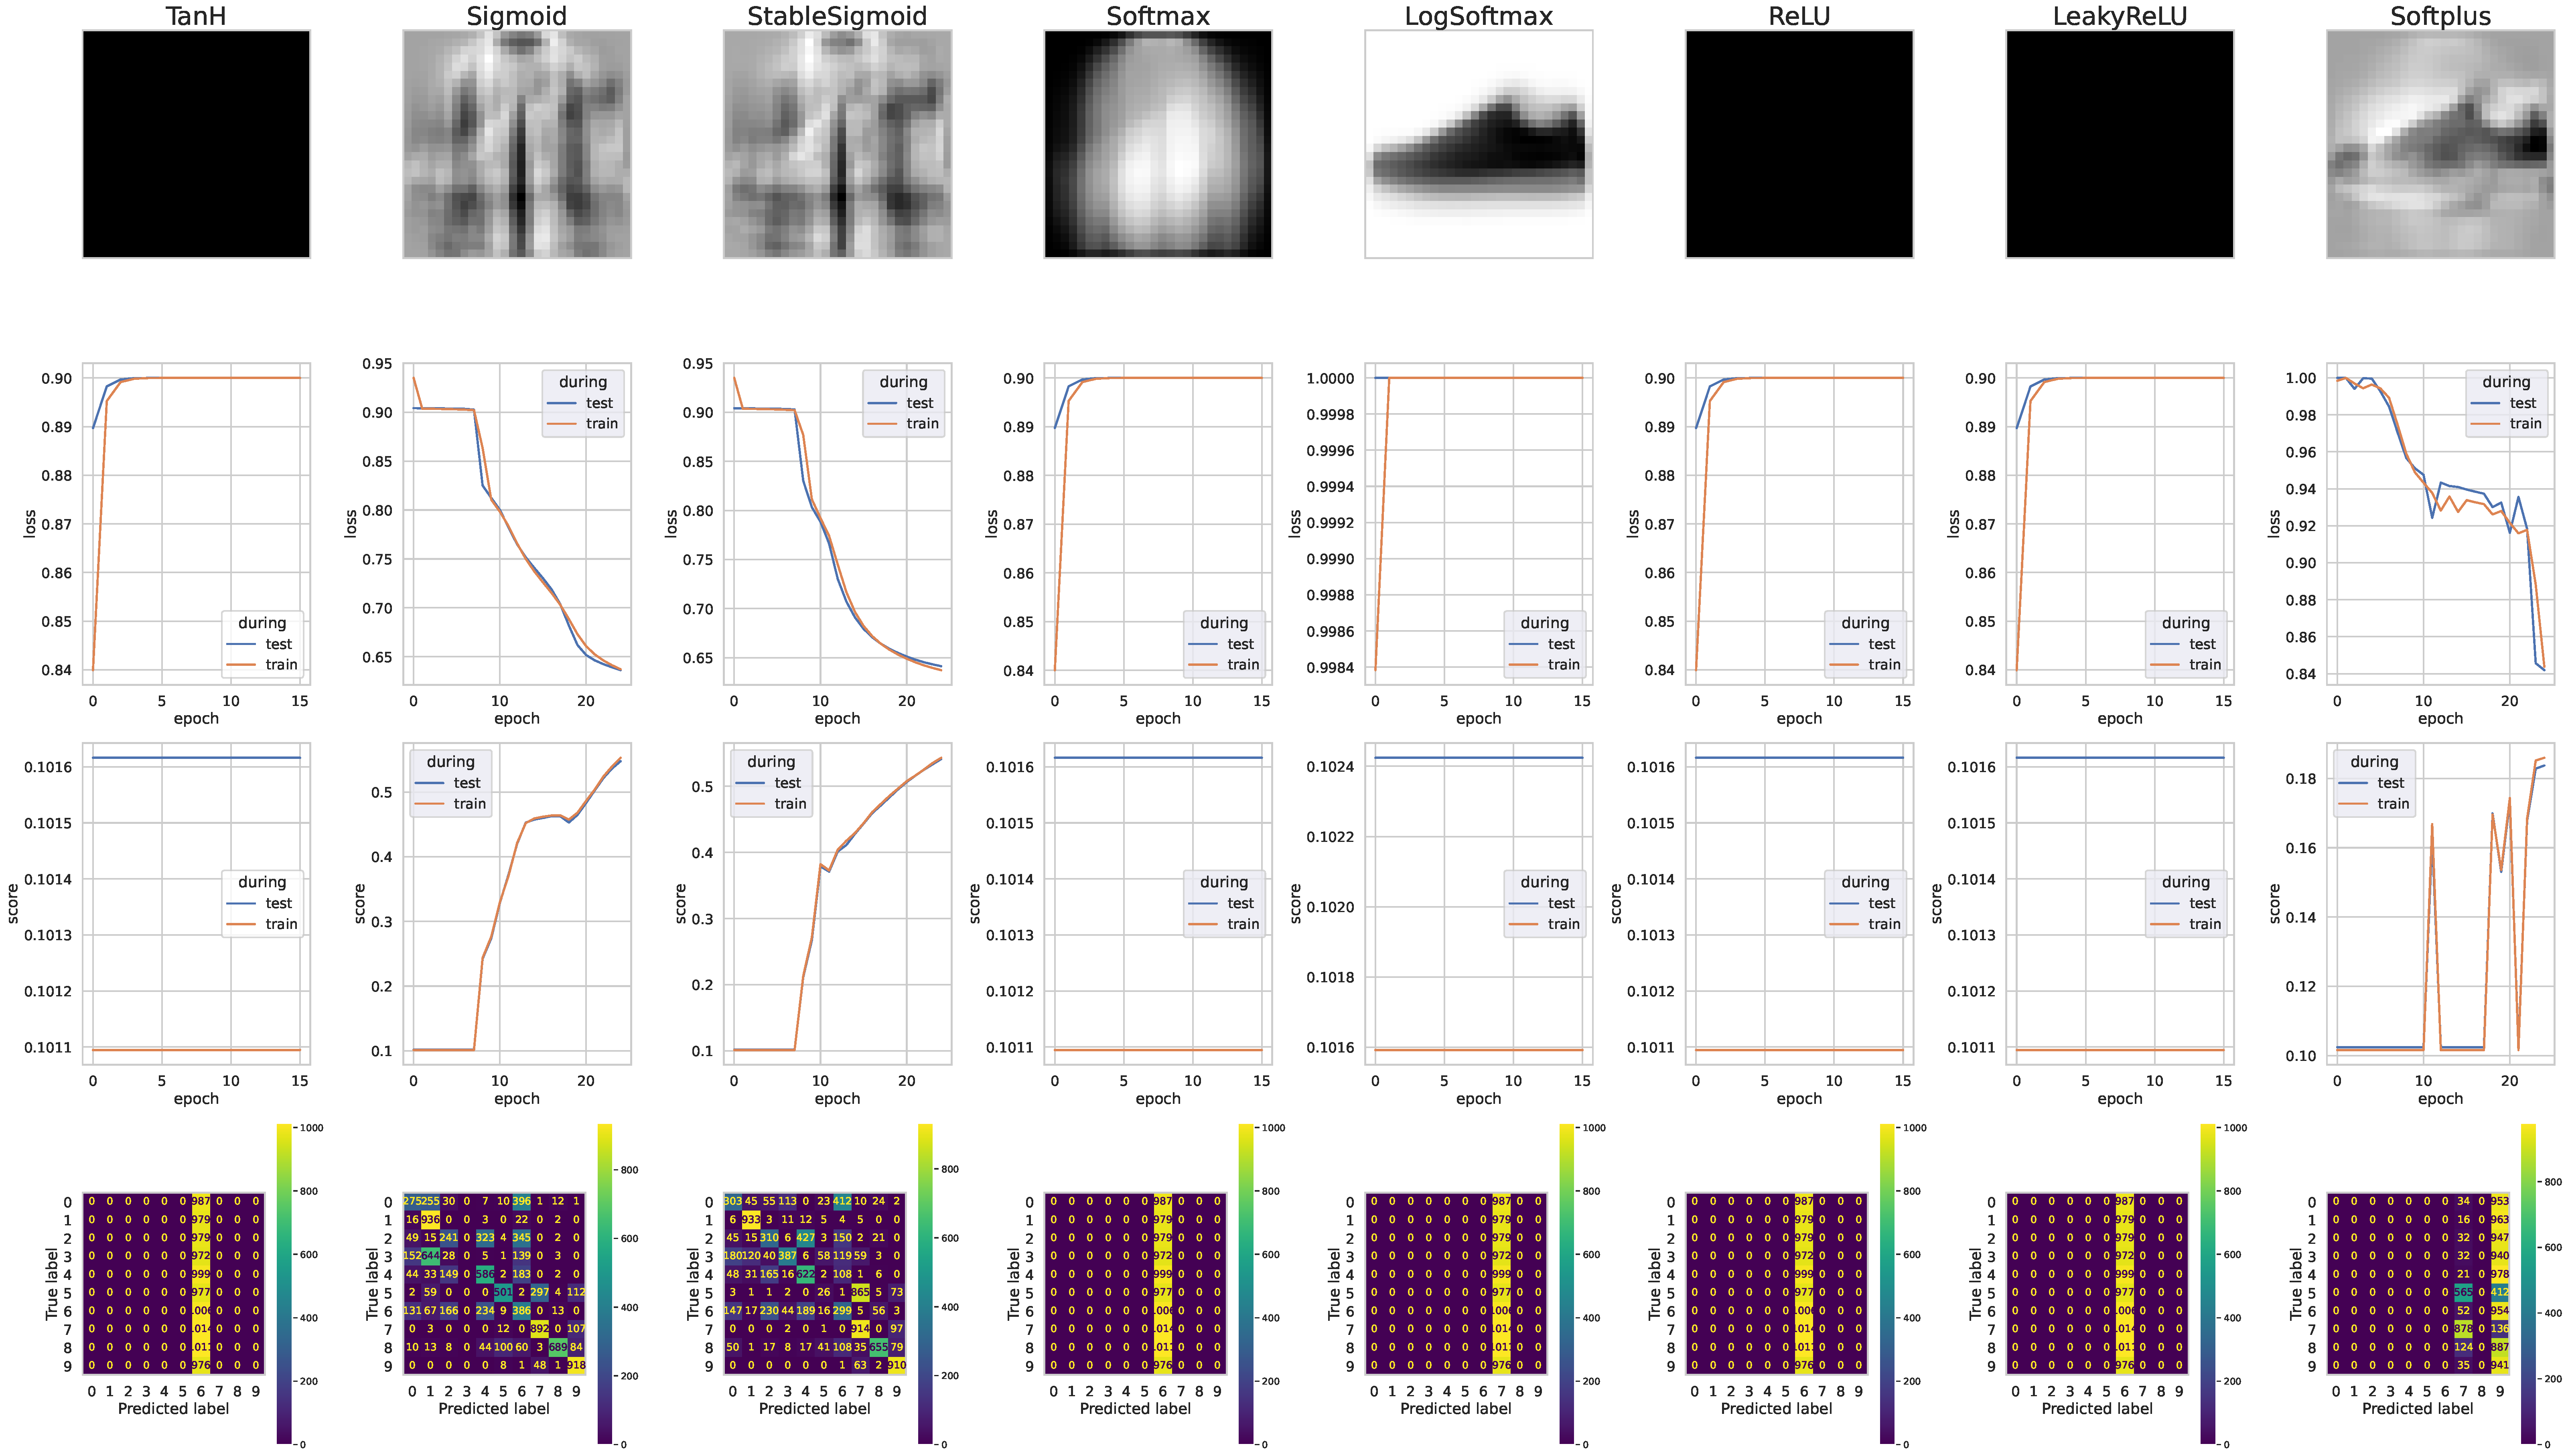
\includegraphics[width=\textwidth]{activation_func.pdf}
    \caption{Représentation des paramètres, de l'évolution du coût et du score par époque en fonction de la fonction d'activation}
    \label{fig:activationfunc}
\end{figure}

\subsection{Classification et convolution}

L'utilisation de réseaux de neurones convolutifs offre de nombreux avantages pour le traitement des images. La convolution permet de capturer des motifs locaux, de réduire le nombre de paramètres à apprendre, d'obtenir une certaine invariance aux translations et de réduire la dimensionnalité des données. Cela en fait un module particulièrement adapté aux images, aux séquences temporelles ou aux signaux.

Nous avons implémenté avec succès la convolution en une dimension, ainsi que les couches de pooling (Max et Average). L'implémentation a été optimisée en utilisant le moins de boucles possible, en se basant sur les fonctionnalités avancées de la bibliothèque \texttt{numpy} (seulement une boucle présente dans la convolution, sur la taille du kernel). Notre raisonnement est détaillé au sein du code.

Un réseau utilisant une seule couche convolutionnelle de ce type \texttt{Conv1D(3,1,32) $\rightarrow$ MaxPool1D(2,2) $\rightarrow$ Flatten() $\rightarrow$ Linear(4064,100) $\rightarrow$ ReLU() $\rightarrow$ Linear(100,10)} fonctionne extrêmement bien dans le cadre de la reconnaissance de chiffres.

En utilisant un batch de taille fixe de 32, 50 époques et un early-stopping à 5, répétées 10 fois, nous obtenons un score d'apprentissage de $99.36 \pm 0.0017~\%$ et un \textbf{score d'évaluation} de $\mathbf{97.08 \pm 0.0016~\%}$, en seulement $31 \pm 6$ époques.

Par ailleurs, l'initialisation des poids est d'une grande importance dans les couches convolutionnelles. Par exemple, une initialisation à zéro ne fonctionne pas (voir figure \ref{fig:convinit}). Dans notre cas, nous avons utilisé une initialisation de Xavier avec une loi normale pour les convolutions, et une initialisation de He normale pour les modules linéaires.

\begin{figure}[htbp]
    \centering
    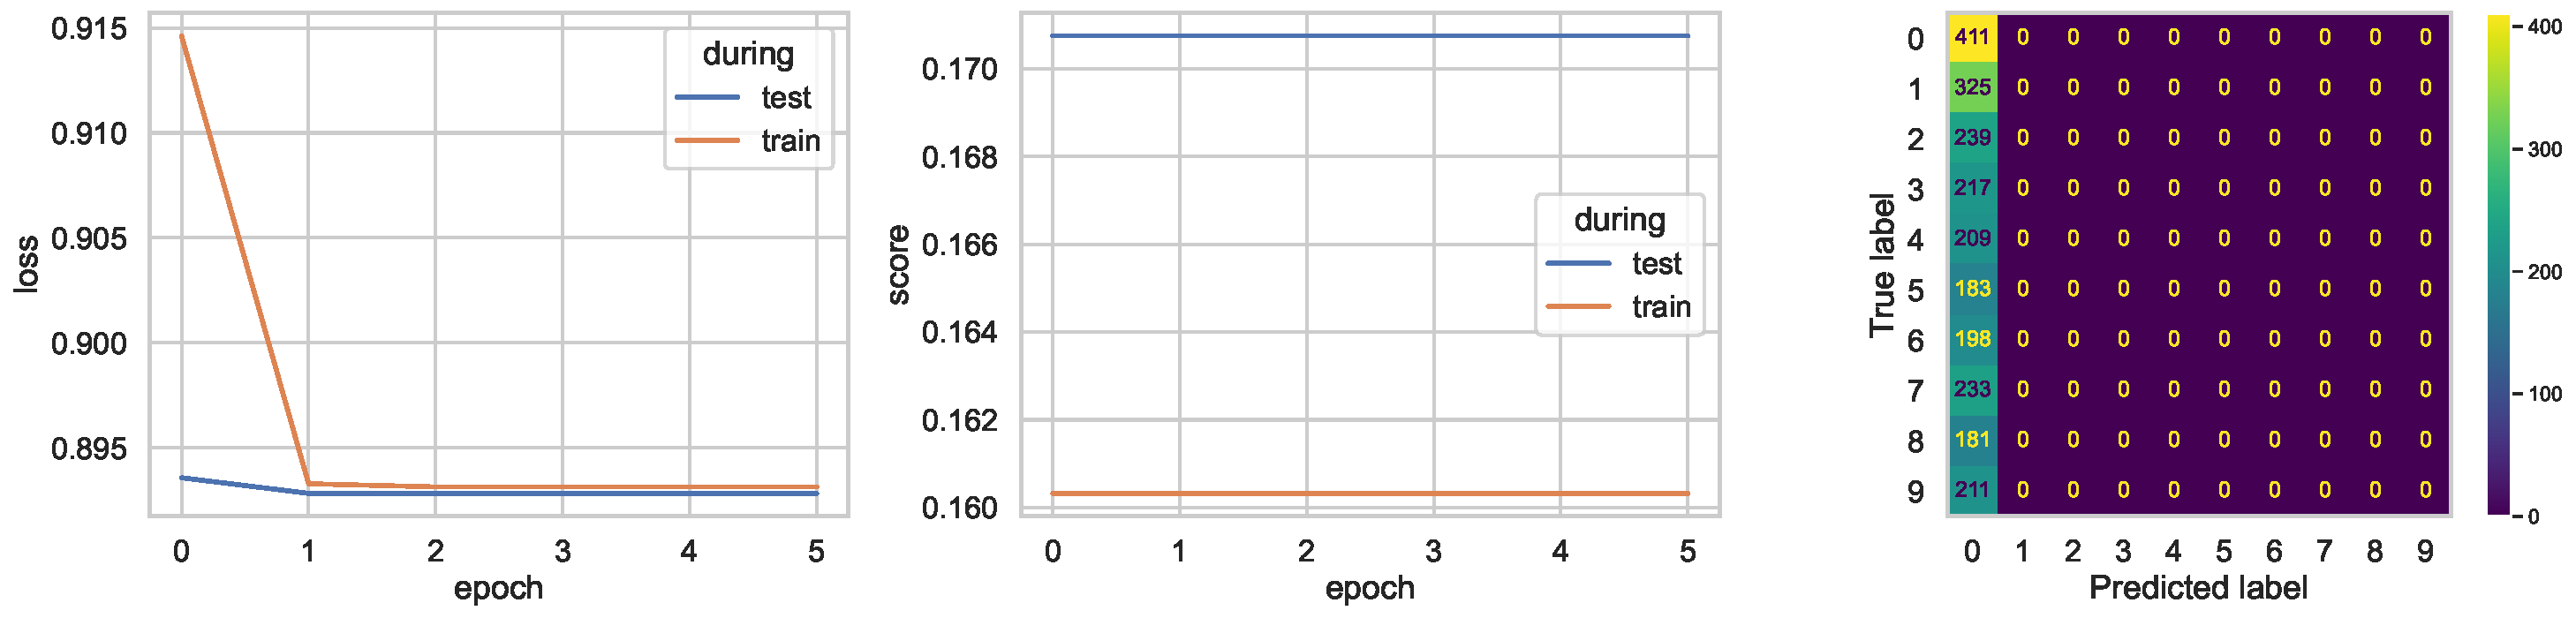
\includegraphics[width=\textwidth]{conv/conv_32batch_zeros.pdf}
    \caption{Impact de l'initialisation des poids à zéros sur un réseau de neurones convolutionnel}
    \label{fig:convinit}
\end{figure}


\subsubsection{Effet de la taille des \textit{batch}}

Le nombre de batchs est un hyperparamètre crucial de notre modèle. Nous observons que de meilleures performances sont obtenues en effectuant l'apprentissage sur des batchs plus petits, ce qui est une pratique courante et bien connue en apprentissage profond. Cependant, cela peut actuellement entraîner un surapprentissage, même si les résultats en évaluation sont bons. De plus, plus la taille du batch est réduite, plus l'apprentissage prendra du temps. Avec des batchs plus grands, le temps d'apprentissage sera considérablement réduit, mais cela peut également avoir un impact sur les instabilités numériques, comme l'explosion du gradient. Ces résultats sont illustrés dans la figure \ref{fig:conv_batch}. Il est important de trouver un équilibre entre la taille du batch, les performances du modèle, la durée de l'apprentissage et les problèmes d'instabilité numérique. Nous utiliserons une taille de batch fixe de 32 pour la suite.


\begin{figure}[htbp]
    \centering
    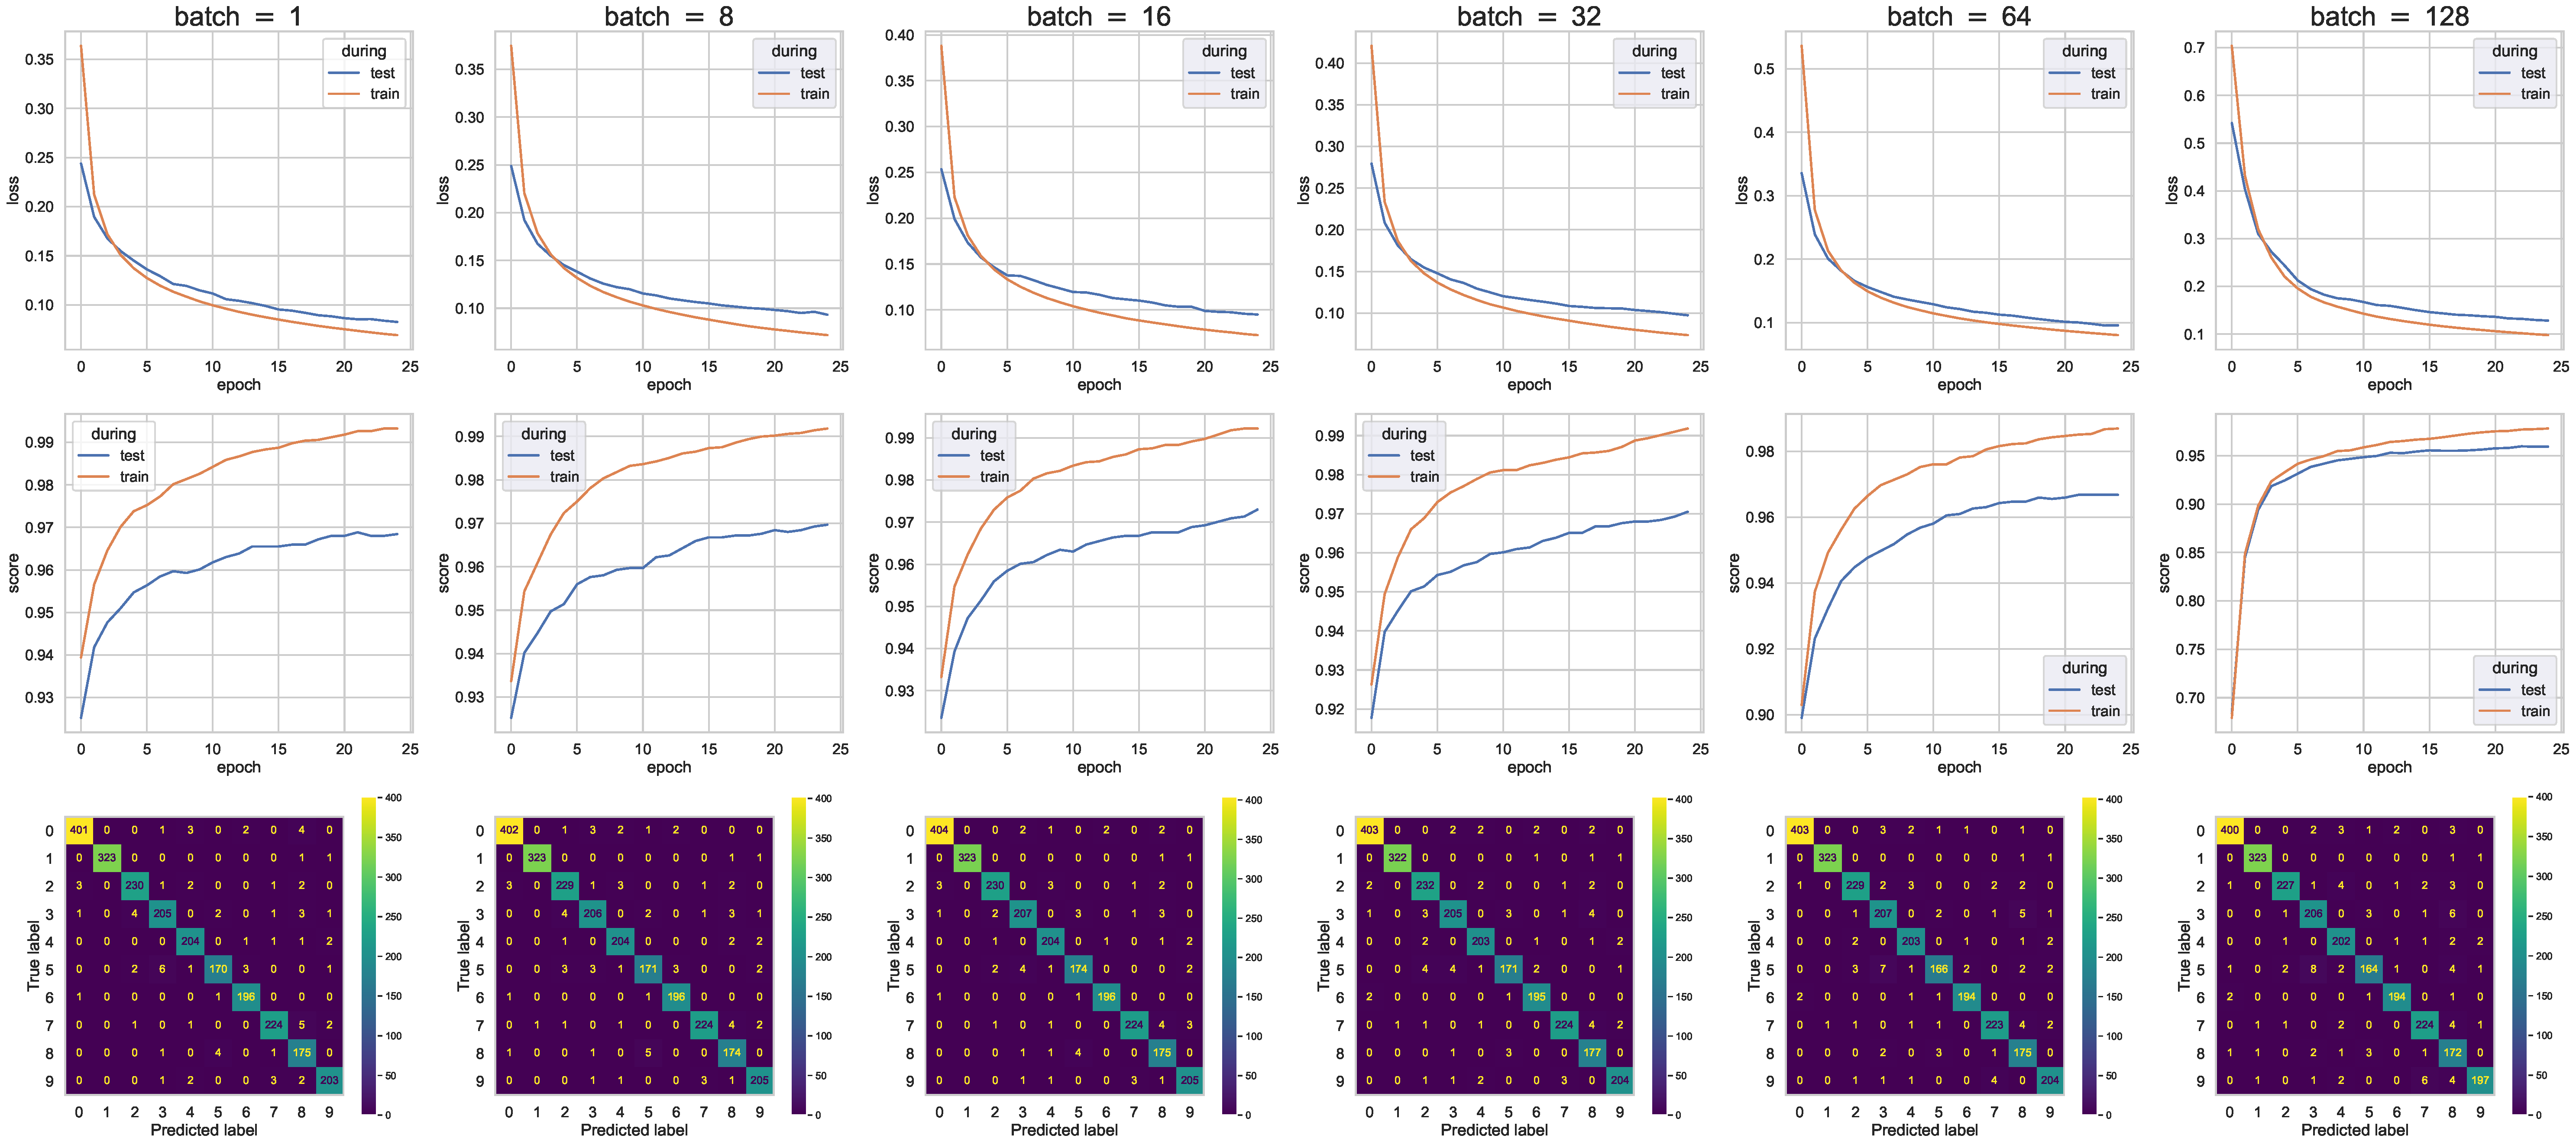
\includegraphics[width=\textwidth]{conv/conv_batch.pdf}
    \caption{Impact de la taille du kernel pour un réseau de neurones convolutionnel}
    \label{fig:conv_batch}
\end{figure}

\subsubsection{Effet de la taille du kernel}

En ajustant la taille du kernel, nous avons la possibilité de capturer des motifs ou des informations à différentes échelles spatiales dans les données. Par exemple, les kernels de petite taille peuvent être efficaces pour détecter des détails fins, tandis que les kernels de plus grande taille sont plus adaptés pour détecter des caractéristiques plus globales. Lors de l'analyse des chiffres manuscrits, ces chiffres sont des éléments cruciaux de l'image, bien que l'image elle-même soit de petite taille. Même en utilisant un kernel de taille 10, qui commence à être relativement grand, les performances restent similaires à celles obtenues avec un kernel de taille 3. Cependant, des problèmes surviennent lorsque nous utilisons un kernel de taille 15 ou plus, ce qui affecte les performances du modèle.

\begin{figure}[htbp]
    \centering
    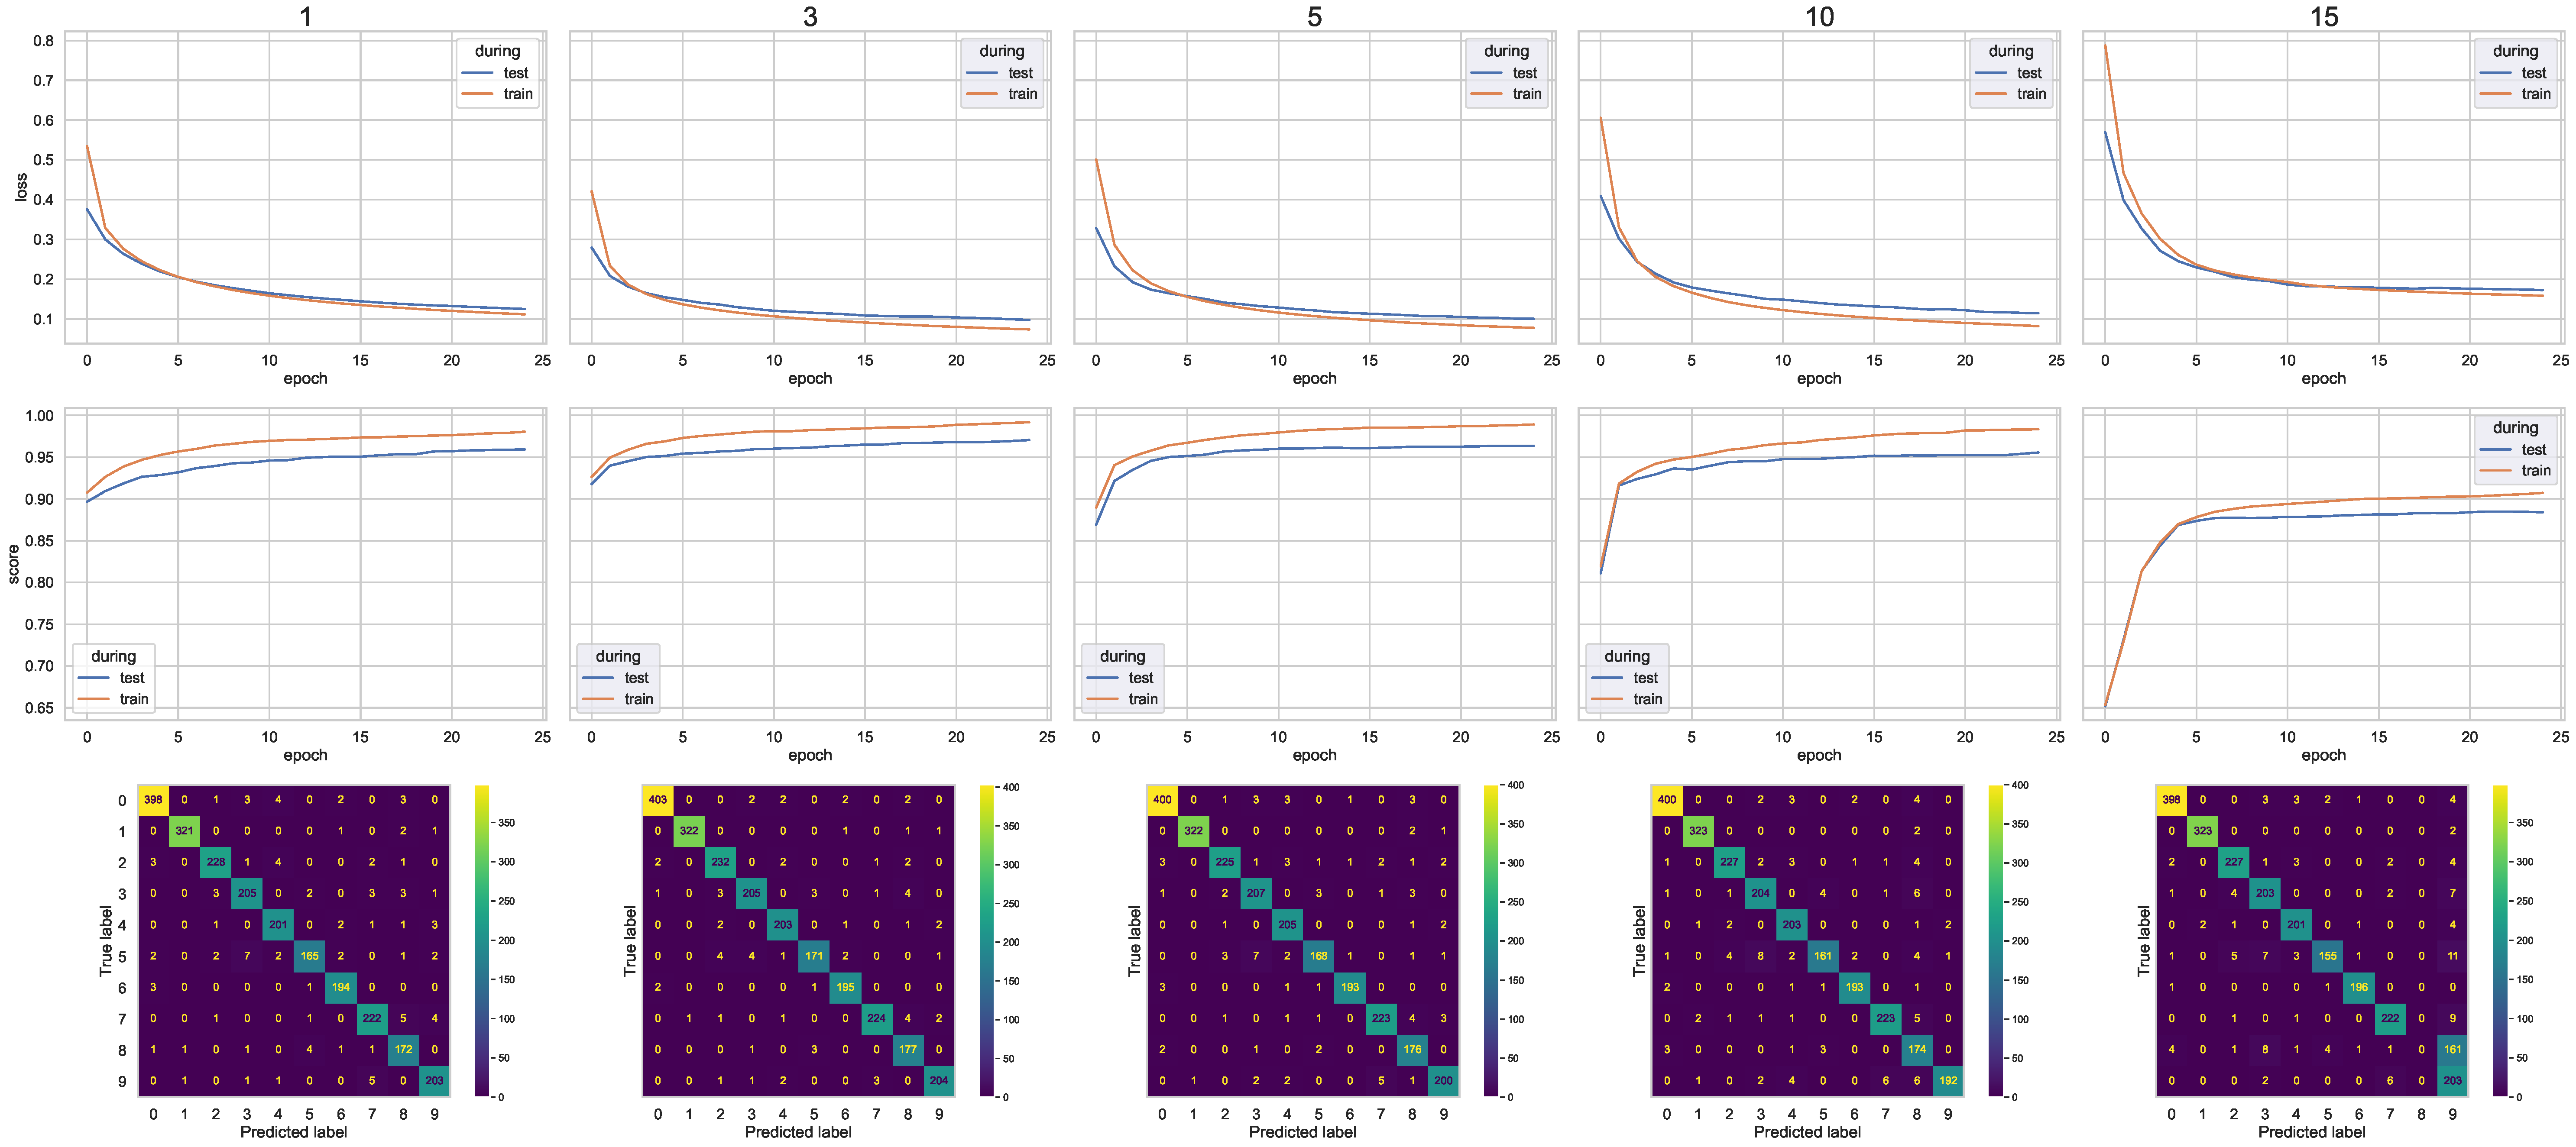
\includegraphics[width=\textwidth]{conv/conv_ksize.pdf}
    \caption{Impact de la taille du kernel pour un réseau de neurones convolutionnel}
    \label{fig:convksize}
\end{figure}

\subsubsection{Effet du nombre de \textit{feature maps}}

Le nombre de \textit{feature maps} dans une couche de convolution joue un rôle crucial dans la capacité du modèle à capturer des caractéristiques et des motifs complexes, ce qui améliore la représentation des données et la capacité de généralisation. Cependant, il est important de trouver un équilibre en tenant compte des contraintes de ressources et des exigences spécifiques du problème. Dans notre cas, nous avons constaté qu'une seule \textit{feature map} était étonnamment suffisante, tandis que 128 \textit{feature maps} fonctionnaient également bien. L'utilisation d'une seule feature map peut être attribuée à la simplicité du problème de reconnaissance de chiffres manuscrits, où les caractéristiques discriminantes peuvent être relativement simples et bien représentées par une seule feature map. En revanche, l'ajout de 128 \textit{feature maps} peut permettre une représentation plus riche et plus complexe des données, ce qui peut être bénéfique pour capturer des détails plus fins ou des motifs plus variés présents dans les images.

\begin{figure}[htbp]
    \centering
    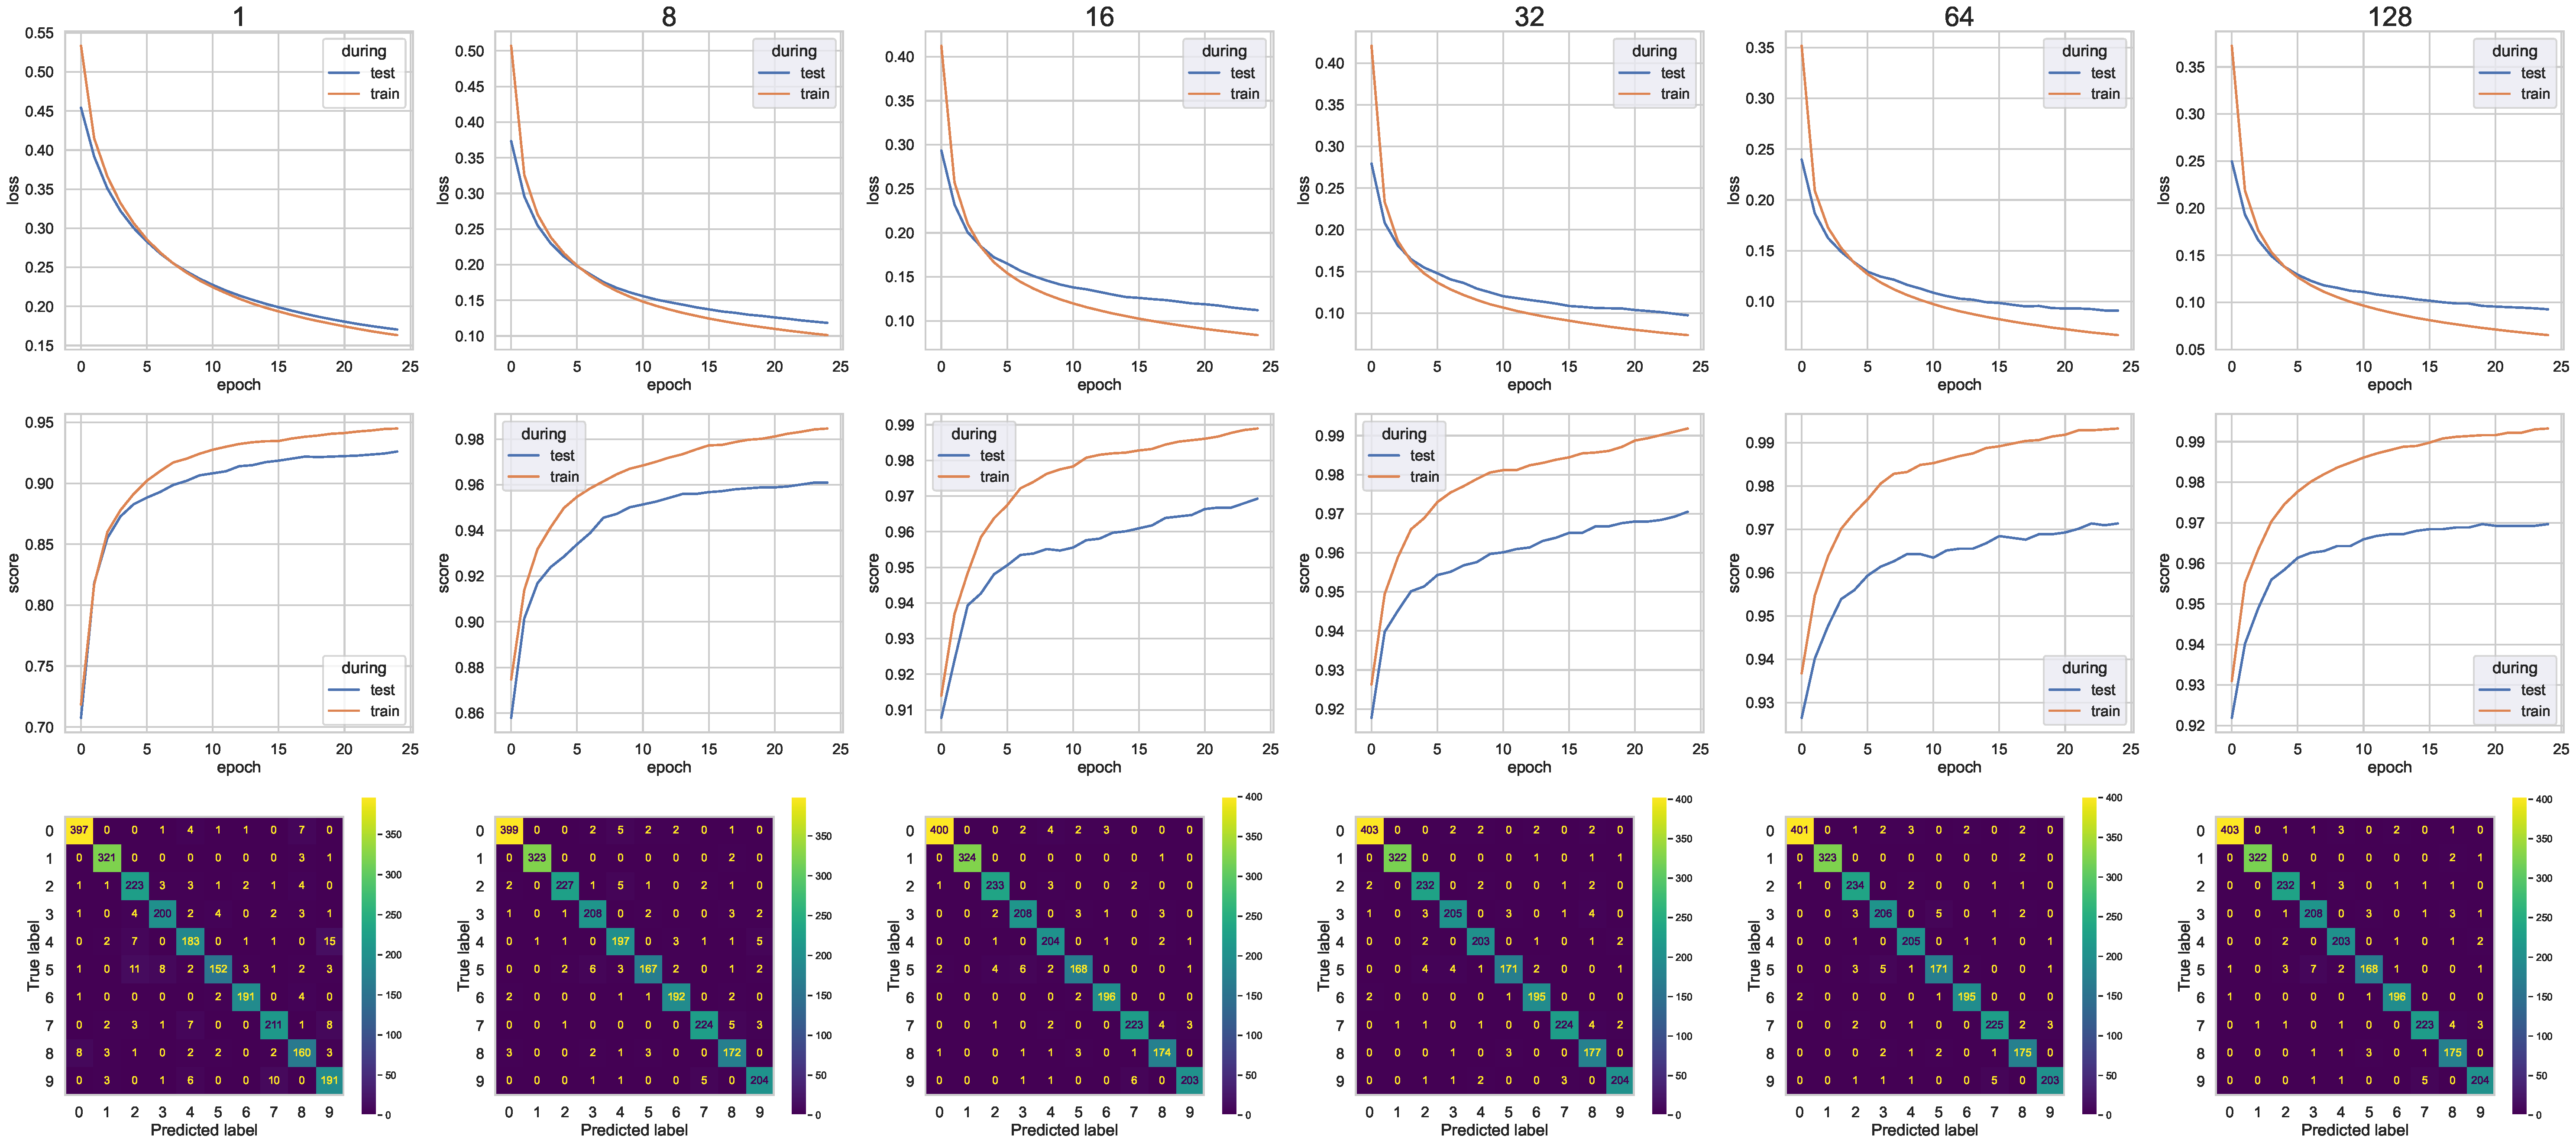
\includegraphics[width=\textwidth]{conv/conv_feature_maps.pdf}
    \caption{Impact du nombre de \textit{feature maps} pour un réseau de neurones convolutionnel}
    \label{fig:convchanout}
\end{figure}

\subsubsection{Diverses architectures}

Nous avons également exploré différentes architectures pour évaluer la robustesse de la convolution, en particulier en augmentant la profondeur des réseaux et en appliquant des fonctions d'activation directement sur les convolutions, comme c'est couramment fait. Cependant, ces variations n'ont pas donné de résultats significativement meilleurs. En fait, nous avons constaté que l'augmentation de la taille du réseau de neurones convolutifs ne se traduit pas nécessairement par une meilleure classification.

L'architecture à deux couches convolutionnelles, représentée par \texttt{Conv1D(3, 1, 32, 1) $\rightarrow$ ReLU() $\rightarrow$ MaxPool1D(2, 2) $\rightarrow$ Conv1D(3, 32, 32) $\rightarrow$ ReLU() $\rightarrow$ MaxPool1D(2, 2) $\rightarrow$ Flatten() $\rightarrow$ Linear(1984, 10)}, a montré des résultats mitigés (figure \ref{fig:conv2layers}), où le réseau commence à apprendre avant de régresser soudainement. Les performances obtenues sont nettement inférieures à celles du réseau précédent, indiquant que l'utilisation d'une seule couche linéaire n'est probablement pas suffisante pour classifier correctement nos données.

\begin{figure}[htbp]
    \centering
    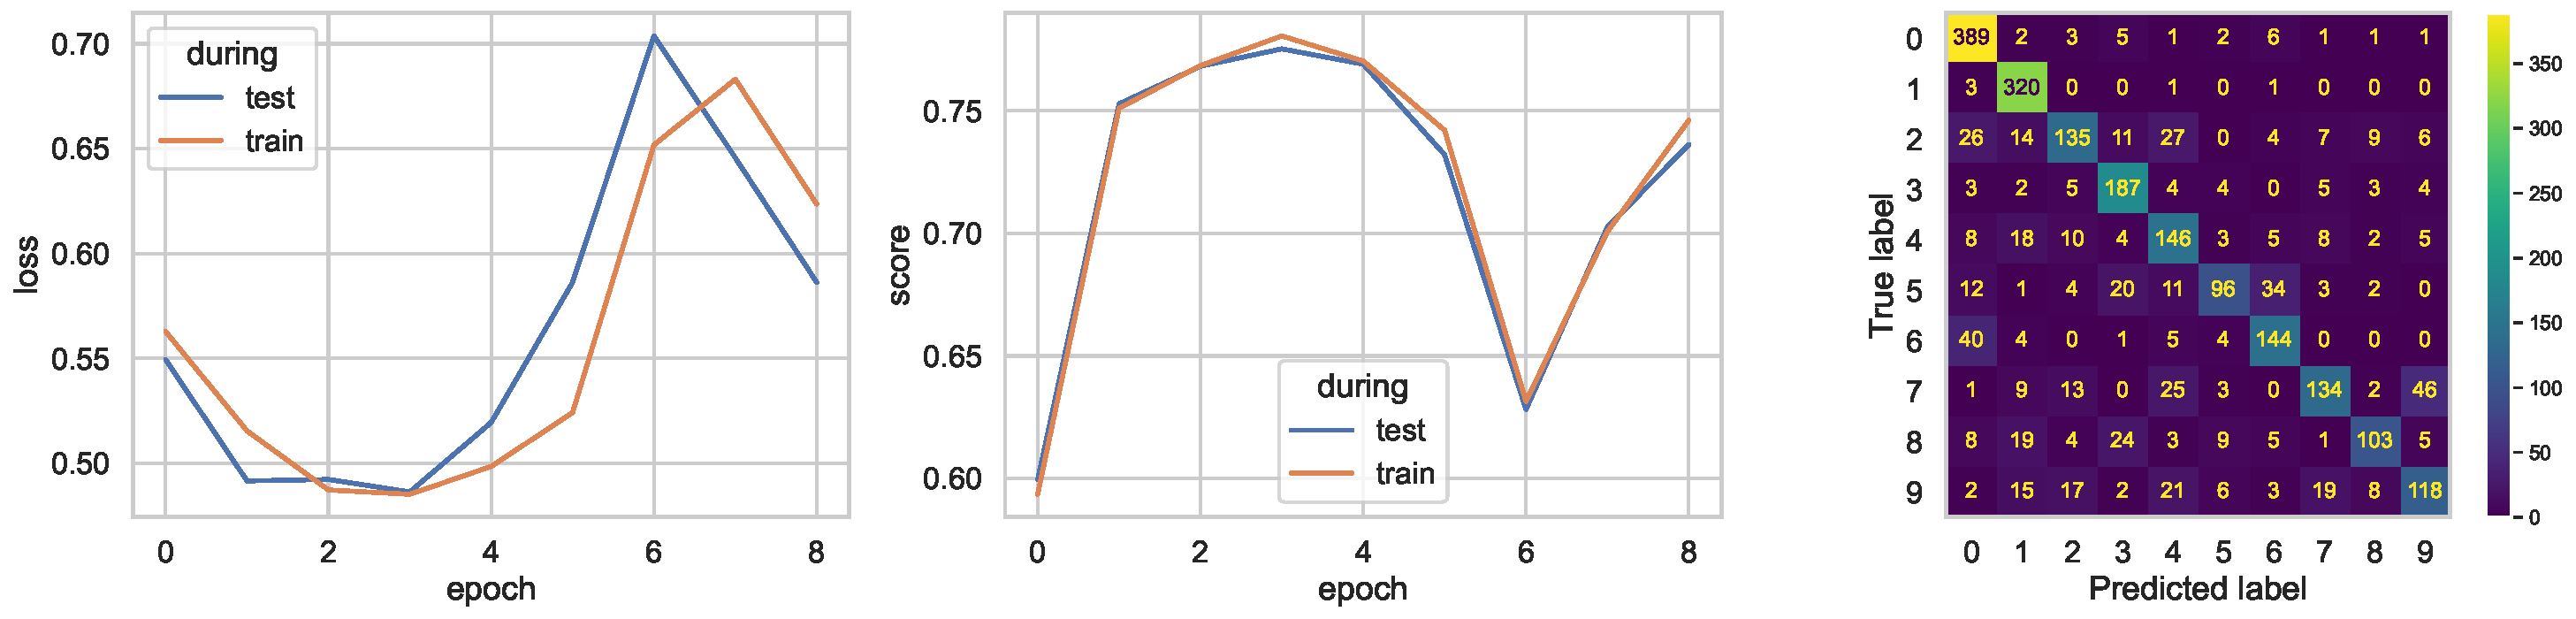
\includegraphics[width=\textwidth]{conv/conv_2layers.pdf}
    \caption{Réseau de neurones convolutionnel à 2 couches}
    \label{fig:conv2layers}
\end{figure}

En ce qui concerne l'architecture à quatre couches convolutionnelles, représentée par \texttt{Conv1D(3, 1, 64, 1) $\rightarrow$ ReLU() $\rightarrow$ MaxPool1D(8, 2) $\rightarrow$ Conv1D(3, 64, 64) $\rightarrow$ ReLU() $\rightarrow$ MaxPool1D(8, 2) $\rightarrow$ Conv1D(3, 64, 64) $\rightarrow$ ReLU() $\rightarrow$ MaxPool1D(8, 2) $\rightarrow$ Conv1D(3, 64, 64) $\rightarrow$ ReLU() $\rightarrow$ MaxPool1D(8, 2) $\rightarrow$ Flatten() $\rightarrow$ Linear(512, 10)}, les résultats (figure \ref{fig:conv4layers}) montrent une meilleure capacité d'apprentissage par rapport au réseau précédent, mais les performances ne sont toujours pas satisfaisantes. Nous avons également observé que la classe 2 est celle qui est la moins bien classée, ce qui contribue à ces performances insuffisantes. Il est possible que la taille du kernel dans la couche de Max Pooling soit trop élevée pour conserver un nombre significatif de features, ce qui empêche une identification précise de cette classe.

\begin{figure}[htbp]
    \centering
    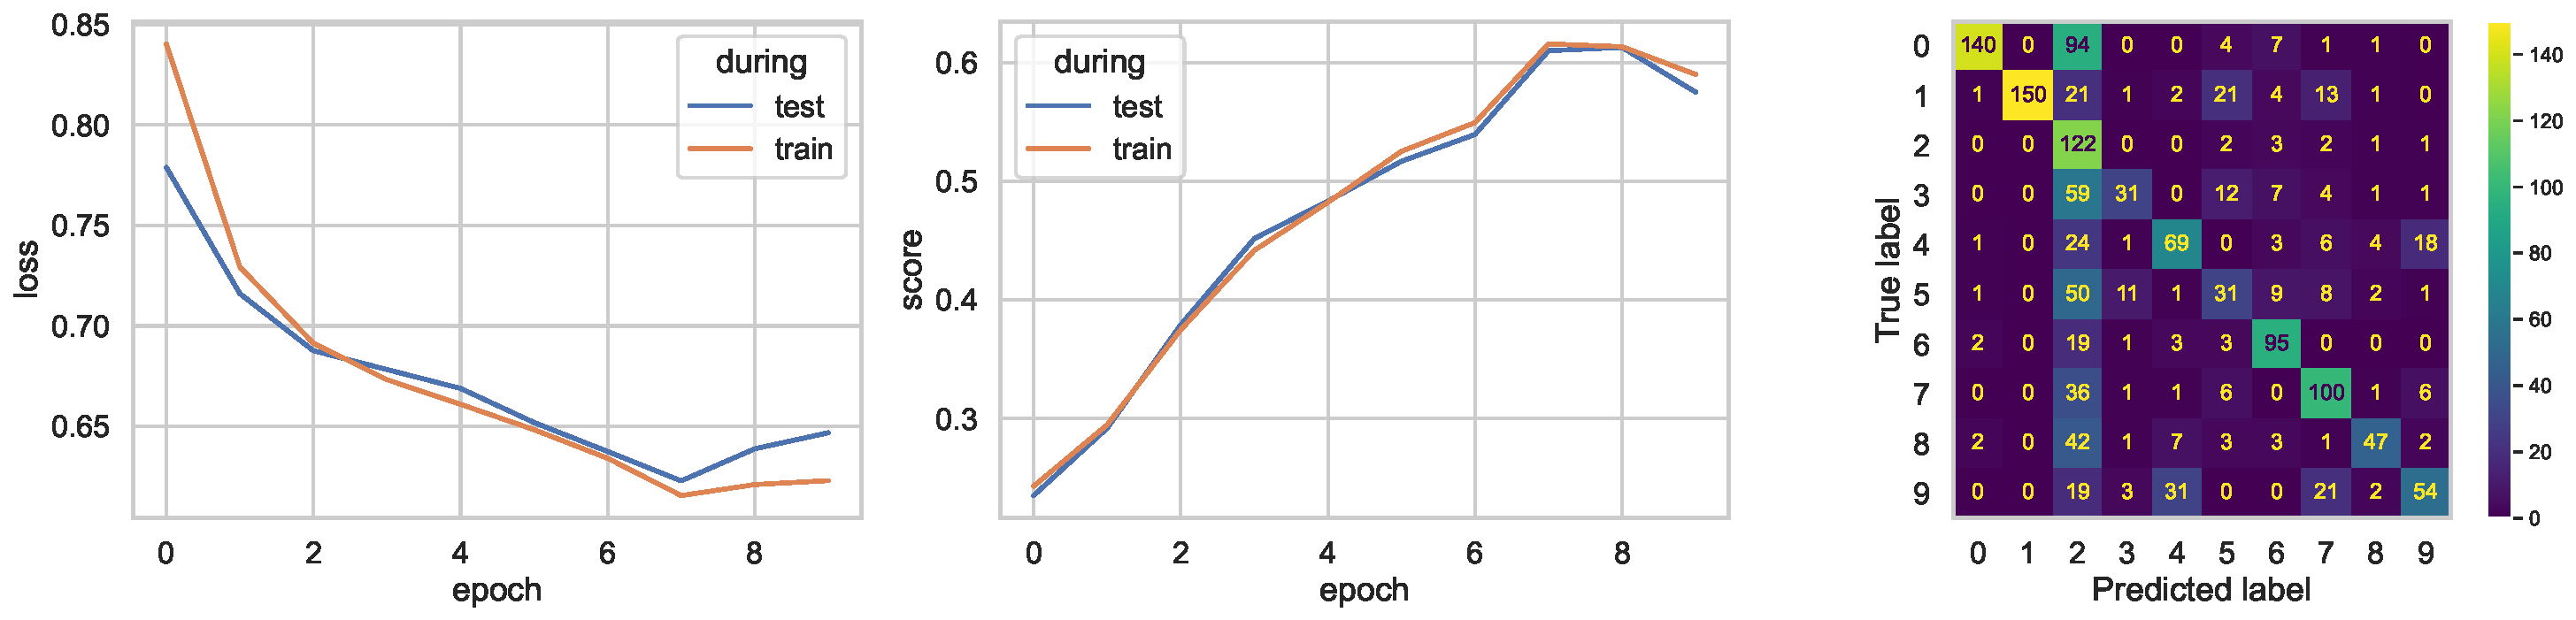
\includegraphics[width=\textwidth]{conv/conv_4layers.pdf}
    \caption{Réseau de neurones convolutionnel à 4 couches}
    \label{fig:conv4layers}
\end{figure}

Un modèle trop complexe n'est donc pas synonyme de bonne performance.

\subsubsection{Et sur \texttt{fashion-mnist} ?}

Atchitecture similaire à précédent :

\begin{figure}[htbp]
    \centering
    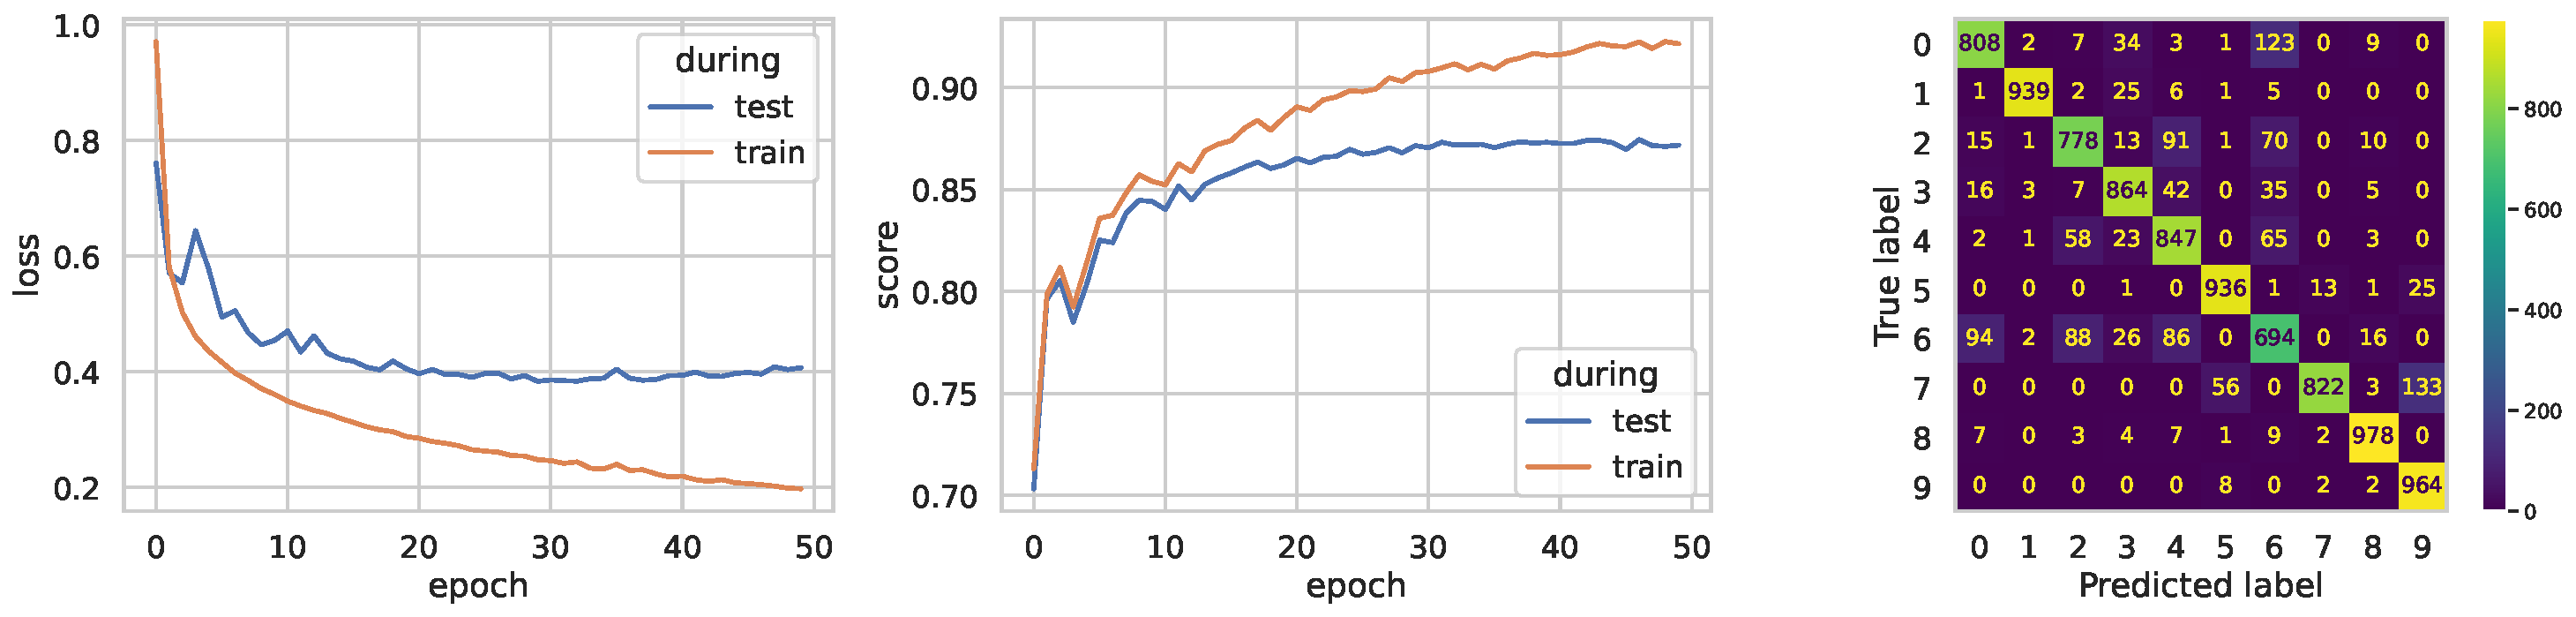
\includegraphics[width=\textwidth]{conv/fashion_conv_1layer_2linear.pdf}
    \caption{Réseau de neurones convolutionnel à 1 couche}
    \label{fig:conv2layers_fashion}
\end{figure}

Avec 3 couches, dans l'optique d'avoir une sortie plus petite dans la première couche linéaire :

\begin{figure}[htbp]
    \centering
    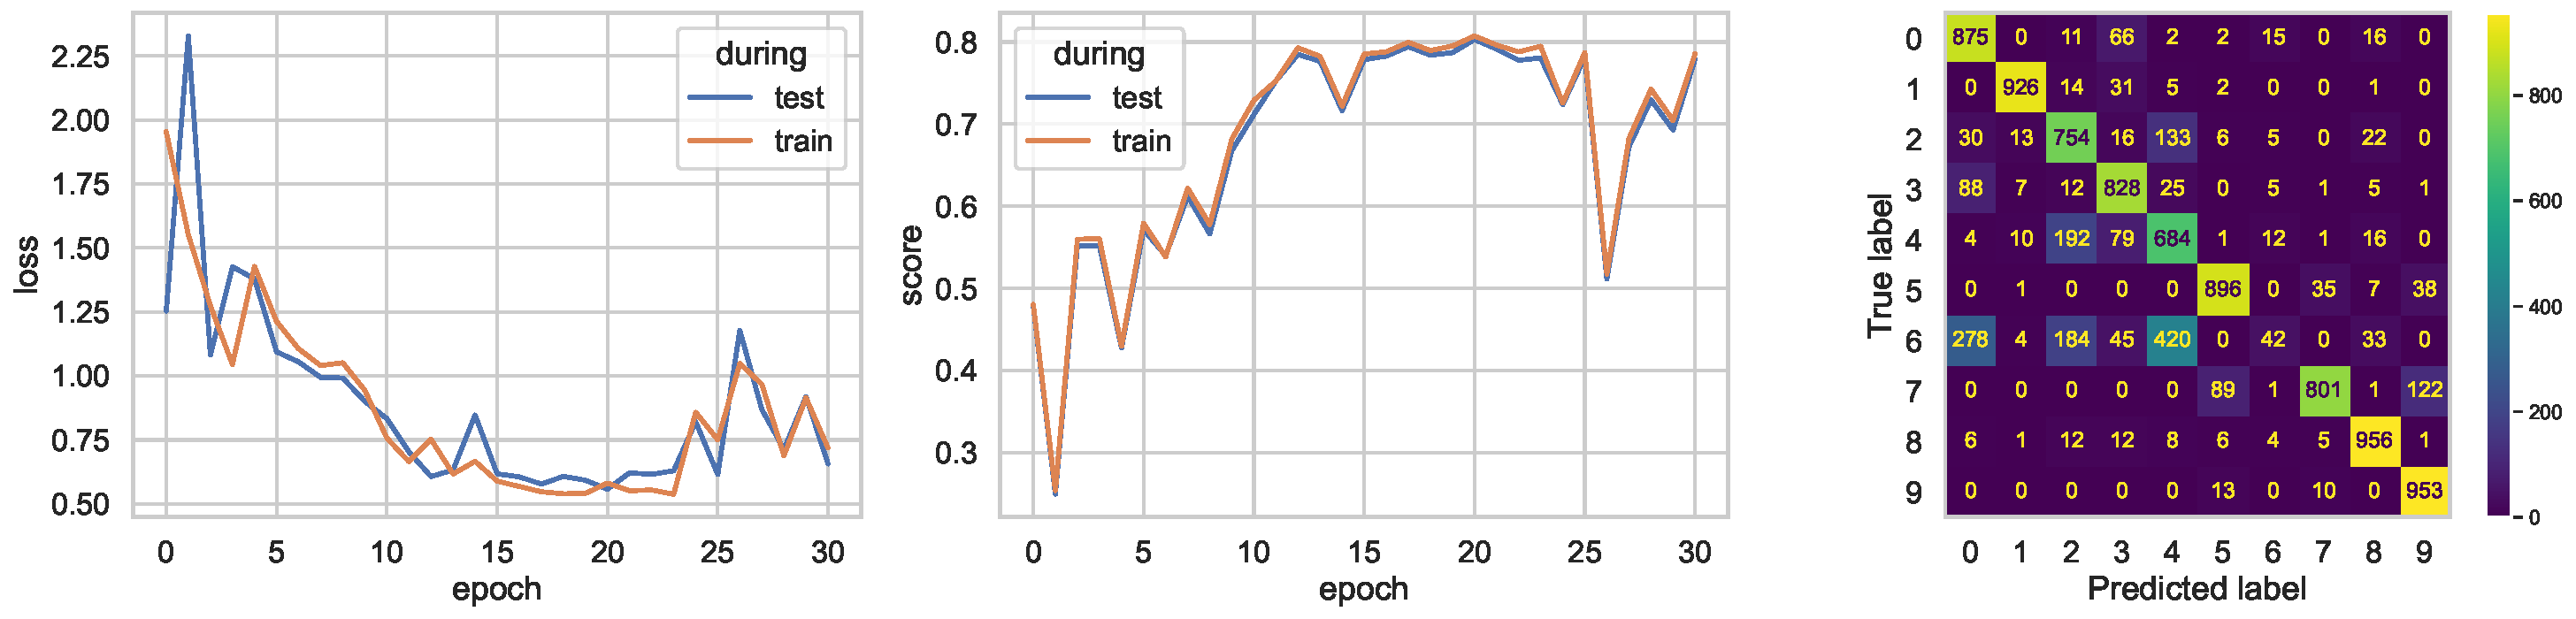
\includegraphics[width=\textwidth]{conv/fashion_conv_3layers_2linear.pdf}
    \caption{Réseau de neurones convolutionnel à 3 couches}
    \label{fig:conv3layers_fashion}
\end{figure}

La convolution n'améliore pas beaucoup les scores de classification sur \texttt{fashion-mnist} (84~\% à un peu plus de 85~\%). Alors que sur \texttt{usps}, l'ajoue d'une couche de convolution permetait de passer de 85~\% à 97~\%.

\subsection{Auto-encodeur}

Nous avons également exploré l'utilisation d'architectures encodeur-décodeur (ou auto-encodeurs), pour des tâches de reconstruction ou de génération de données.

\subsubsection{Reconstruction}

Dans notre cas, nous avons entraîné un modèle pour reconstruire les images d'origine à partir de leur représentation latente. L'encodeur prend les images en entrée et les transforme en une représentation latente de dimension réduite. Ensuite, le décodeur prend cette représentation latente et tente de générer des images similaires aux images d'origine. L'objectif de cette expérience était d'évaluer la capacité du modèle à capturer les caractéristiques distinctives des images et à reconstruire des images de qualité. La performance du modèle peut être évaluée en mesurant la différence entre les images reconstruites et les images d'origine.

De plus, l'architecture de l'encodeur-décodeur peut également être utilisée pour générer de nouvelles images similaires à celles du jeu de données MNIST : en fournissant une représentation latente aléatoire au décodeur, il est possible de générer de nouvelles images qui ressemblent aux images du jeu de données.

Nous avons entrainé un auto-encodeur sur les deux jeux de données précédents (\texttt{USPS} et \texttt{fashion-mnist}). 

\paragraph*{\texttt{fashion-mnist}}

Dans le cas du jeu de données \texttt{fashion-mnist}, nous avons testé trois architectures pour l'auto-encodeur :

\begin{enumerate}
    \item \label{reseau1} \texttt{Linear(784, 64) $\rightarrow$ TanH() $\rightarrow$ Decoder} 
    \item \texttt{Linear(784, 256) $\rightarrow$ TanH() $\rightarrow$ Linear(256, 64) $\rightarrow$ TanH() $\rightarrow$ Decoder}
    \item \texttt{Linear(784, 512) $\rightarrow$ TanH() $\rightarrow$ Linear(512, 256) $\rightarrow$ TanH() $\rightarrow$ Linear(256, 128) $\rightarrow$ TanH() $\rightarrow$ Linear(128, 64) $\rightarrow$ TanH() $\rightarrow$ Decoder}
\end{enumerate}

\texttt{Decoder} représente l'architecture transposée du réseau avec une \texttt{Sigmoid()} en sortie et l'utilisation d'une \texttt{BCELoss}. 

Ces trois architectures, de complexité croissante, ont toutes conduit à une stagnation rapide du coût d'évaluation pendant l'entraînement (figure \ref{fig:lossencoder}). Cette valeur varie légèrement en fonction de la complexité du réseau. Dans la figure \ref{fig:reconstruction}, nous pouvons effectivement constater que la précision de la reconstruction des images s'est améliorée à mesure que la complexité du réseau augmentait, ce qui suggère que des architectures plus complexes sont capables de capturer et de reconstruire les caractéristiques distinctives des images avec une meilleure fidélité.

\begin{figure}[htbp]
    \centering
    \includegraphics*[width=.85\textwidth]{loss_encoder_fashion_3_networks.pdf}
    \caption{Coût cross-entropique binaire, pour chaque modèle, sur 30 époques}
    \label{fig:lossencoder}
\end{figure}

\begin{figure}[htbp]
    \centering
    \includegraphics*[width=.85\textwidth]{reconstruction_per_network_cplxity.pdf}
    \caption{Exemple de reconstruction en fonction de la complexité du réseau}
    \label{fig:reconstruction}
\end{figure}

Pour le réseau n°~1, une étude de l'influence de la fonction d'activation placée avant l'espace latent a été réalisée. Le réseau a donc la forme suivante : \texttt{Linear(784, 64) $\rightarrow$ Activation() $\rightarrow$ Decoder}. Les résultats sont présentés dans la figure \ref{fig:accfct}. 

\begin{figure}[htbp]
    \centering
    \includegraphics*[width=\textwidth]{encoder_decoder_middle_func_simple_net.pdf}
    \caption{Fonction de coût et reconstruction pour une architecture de type réseau n°~1}
    \label{fig:accfct}
\end{figure}

Il est observé que les fonctions d'activation \texttt{Softmax()} et \texttt{LogSoftmax()} rencontrent des difficultés d'apprentissage importantes. De plus, la fonction d'activation \texttt{ReLU} apprend moins rapidement que les autres fonctions d'activation.

Sur les figures \ref{fig:perEpochSimple} et \ref{fig:perEpochBig}, nous nous sommes également amusés à visualiser la reconstruction de l'image au fil des époques d'apprentissage, afin d'observer l'évolution de la qualité de la reconstruction à mesure que le modèle apprend.

\begin{figure}[htbp]
    \centering
    \includegraphics*[width=\textwidth]{reconstruction_per_epoch_simple_model.pdf}
    \caption{Reconstruction par époque pour le modèle n°~1}
    \label{fig:perEpochSimple}
\end{figure}

\begin{figure}[htbp]
    \centering
    \includegraphics*[width=\textwidth]{reconstruction_per_epoch_big_model.pdf}
    \caption{Reconstruction par époque pour le modèle n°~3}
    \label{fig:perEpochBig}
\end{figure}

\subsubsection{Organisation de l'espace latent}

Afin de visualiser l'espace latent de 64 dimensions, nous avons utilisé l'algorithme t-SNE pour le réduire à deux dimensions afin de le rendre visualisable. Cette procédure a été appliquée aux deux jeux de données et à chaque ensemble d'entraînement et de test, en utilisant l'auto-encodeur avec le plus de paramètres. Les t-SNE sur le jeu de test présentent des similarités avec ceux du jeu d'entraînement, et nous présenterons ici uniquement les visualisations des données d'entraînement, illustrées par les figures \ref{fig:tsneMnist} et \ref{fig:tsneUsps}.

\begin{figure}[htbp]
    \centering
    \includegraphics*[width=.75\textwidth]{tsne_mnist_train_big.pdf}
    \caption{t-SNE sur l'espace latent du modèle n°~3 pour \texttt{fashion-mnist} en utilisant les données d'entrainement}
    \label{fig:tsneMnist}
\end{figure}

\begin{figure}[htbp]
    \centering
    \includegraphics*[width=.75\textwidth]{tsne_usps_train_big.pdf}
    \caption{t-SNE sur l'espace latent d'un plus gros modèle pour \texttt{USPS} en utilisant les données d'entrainement}
    \label{fig:tsneUsps}
\end{figure}

Les résultats sont plutôt intéressants. En effet, on observe que les classes 0, 2, 4 et 6 ne forment pas vraiment des groupes distincts. Ces classes correspondent respectivement aux T-shirts/hauts, aux pulls, aux manteaux et aux chemises. Les classes des hauts étant visuellement similaires, ces classes se mélangent davantage lors de la réduction à deux dimensions. En revanche, des classes telles que les pantalons (classe 1) ou les chaussures (classe 5) ont des caractéristiques plus distinctes, ce qui les rend plus facilement discernables dans l'espace latent réduit.


\subsubsection{Débruitage}

Notre objectif est de générer des versions débruitées des images d'origine, ce qui équivaut à un travail de restauration / reconstruction. Cela démontre la capacité du modèle à éliminer le bruit et à récupérer les informations essentielles des images initiales. Les trois modèles précédemment entraînés ont été utilisés pour cette tâche.

En appliquant un bruit gaussien de 20 \% sur une image de chaque classe, le modèle le plus simple, présenté dans la figure \ref{fig:reconstruct_noisy_all_small}, s'en sort plutôt bien. Bien qu'il y ait une perte d'informations, notamment au niveau des contours, il parvient à retrouver la forme générale de chaque classe tout en préservant fidèlement les niveaux de gris. Il reste donc limité quant à la capture des détails fins des images.

\begin{figure}[htbp]
    \centering
    \includegraphics*[width=\textwidth]{reconstruct_noisy_all_simple.pdf}
    \caption{Reconstruction d'une image bruitée de chaque classe pour le réseau n° 1}
    \label{fig:reconstruct_noisy_all_small}
\end{figure}

Le deuxième modèle, illustré dans la figure \ref{fig:reconstruct_noisy_all_medium}, offre de meilleures performances en termes de reconstruction en parvenant à identifier plus précisément les contours et les couleurs des objets. Néanmoins, il présente quelques difficultés avec certaines classes, comme la confusion entre les chaussures de tennis (classe 7) et les talons, ce qui peut être attribué à une similarité visuelle entre ces deux catégories.

\begin{figure}[htbp]
    \centering
    \includegraphics*[width=\textwidth]{reconstruct_noisy_all_medium.pdf}
    \caption{Reconstruction d'une image bruitée de chaque classe pour le réseau n° 2}
    \label{fig:reconstruct_noisy_all_medium}
\end{figure}

Le troisième modèle, représenté dans la figure \ref{fig:reconstruct_noisy_all_big}, obtient les meilleurs résultats de reconstruction. Ce modèle parvient à supprimer efficacement le bruit et à retrouver les informations essentielles des images d'origine, offrant ainsi une meilleure fidélité visuelle dans la reconstruction et démontrant sa capacité à apprendre des représentations plus riches et détaillées.

\begin{figure}[htbp]
    \centering
    \includegraphics*[width=\textwidth]{reconstruct_noisy_all_big.pdf}
    \caption{Reconstruction d'une image bruitée de chaque classe pour le réseau n° 3}
    \label{fig:reconstruct_noisy_all_big}
\end{figure}

Les figures \ref{fig:reconstructnoisychaussure}, \ref{fig:reconstructnoisybag}, \ref{fig:reconstructnoisypantalon}, \ref{fig:reconstructnoisycoat} présentent les résultats d'une expérience où nous avons introduit différents niveaux de bruit gaussien pour évaluer la robustesse des modèles de reconstruction. Les images débruitées montrent souvent une perte de fidélité aux images originales, avec une tendance à reconnaître des traits caractéristiques des vestes ou des t-shirts plutôt que de préserver les détails spécifiques de chaque classe. Ces résultats soulignent les limites des modèles lorsqu'ils sont confrontés à des niveaux de bruit élevés et mettent en évidence la difficulté de supprimer efficacement le bruit tout en conservant les caractéristiques distinctives des images d'origine.

\begin{figure}[htbp]
    \centering
    \includegraphics*[width=\textwidth]{reconstruct_noisy_chaussure.pdf}
    \caption{Reconstruction d'une image bruitée de chaussure}
    \label{fig:reconstructnoisychaussure}
\end{figure}

\begin{figure}[htbp]
    \centering
    \includegraphics*[width=\textwidth]{reconstruct_noisy_sac.pdf}
    \caption{Reconstruction d'une image bruitée de sac}
    \label{fig:reconstructnoisybag}
\end{figure}


\begin{figure}[htbp]
    \centering
    \includegraphics*[width=\textwidth]{reconstruct_noisy_pantalon.pdf}
    \caption{Reconstruction d'une image bruitée de pantalon}
    \label{fig:reconstructnoisypantalon}
\end{figure}


\begin{figure}[htbp]
    \centering
    \includegraphics*[width=\textwidth]{reconstruct_noisy_coat.pdf}
    \caption{Reconstruction d'une image bruitée de manteau}
    \label{fig:reconstructnoisycoat}
\end{figure}

Une amélioration significative de l'auto-encodeur peut être obtenue en utilisant des réseaux de neurones convolutionnels qui nécessitent des couches de convolutions transposées pour "déconvolutionner" les données ou des fonctions d'upsampling. 
Une approche plus simple serait d'utiliser une convolution en 2D. Le \textit{padding} serait également nécessaire pour garder la taille d'origine des données.

Nous avons tenté, sans succés, d'utiliser un auto-encodeur avec une architecture utilisant des convolutions 1D de la forme : \texttt{Conv1D(3, 1, 32) $\rightarrow$ ReLU() $\rightarrow$ MaxPool1D(2, 1) $\rightarrow$ Conv1D(3, 32, 16) $\rightarrow$ ReLU() $\rightarrow$ MaxPool1D(2, 1) $\rightarrow$ Conv1D(3, 16, 16) $\rightarrow$ ReLU() $\rightarrow$ Conv1D(2, 16, 32) $\rightarrow$ ReLU() $\rightarrow$ Conv1D(2, stride=2) $\rightarrow$ Sigmoid()}. 

\section{Conclusion}

L'implémentation de cette bibliothèque de deep learning a été une expérience enrichissante, nous offrant une compréhension approfondie des concepts algébriques et de la beauté de la rétropropagation. Bien que nous ayons exploré différentes tâches telles que la reconstruction d'images et la génération de données, nous n'avons malheureusement pas eu le temps d'implémenter des fonctionnalités plus avancées telles que le transfert de style ou la traduction avec un auto-encodeur. 

Cependant, nous reconnaissons l'importance de l'optimisation matérielle, telle que l'utilisation de GPU et la compilation pour améliorer les performances de nos modèles. Cela aurait pu accélérer les calculs et nous permettre d'explorer des architectures plus complexes et des ensembles de données plus volumineux. 

En conclusion, bien que notre exploration ait été limitée par des contraintes de temps, cette expérience nous a permis de mieux comprendre les fondements du deep learning et de réaliser l'importance des choix d'architecture, d'optimisation matérielle et de l'implémentation de fonctionnalités avancées pour atteindre de meilleures performances et explorer des domaines plus vastes.

\end{document}